\chapter{Models on the Hourly Consumption}
\label{chap: hourly}
In this section a more detailed look at the hourly consumption will be provided. It will be investigated how the consumption is distributed over the course of the day, and what the main differences are between the winter and the summer periods. The main goal is to get an alternative estimate of the effect of the temperature on a house. A model based on hourly data might be able to catch variations that are not present in the daily data. The type of model that will be applied is an ARIMAX model, that analyses the data as a time series. Different ARIMAX models will be investigated, it will be tested if the models can make reasonable predictions of a short period with unknown data, and the step response of the models will be calculated. This can be related to the temperature coefficients in the daily models, and the uncertainty of the two will be compared.
\begin{figure}
    \centering
    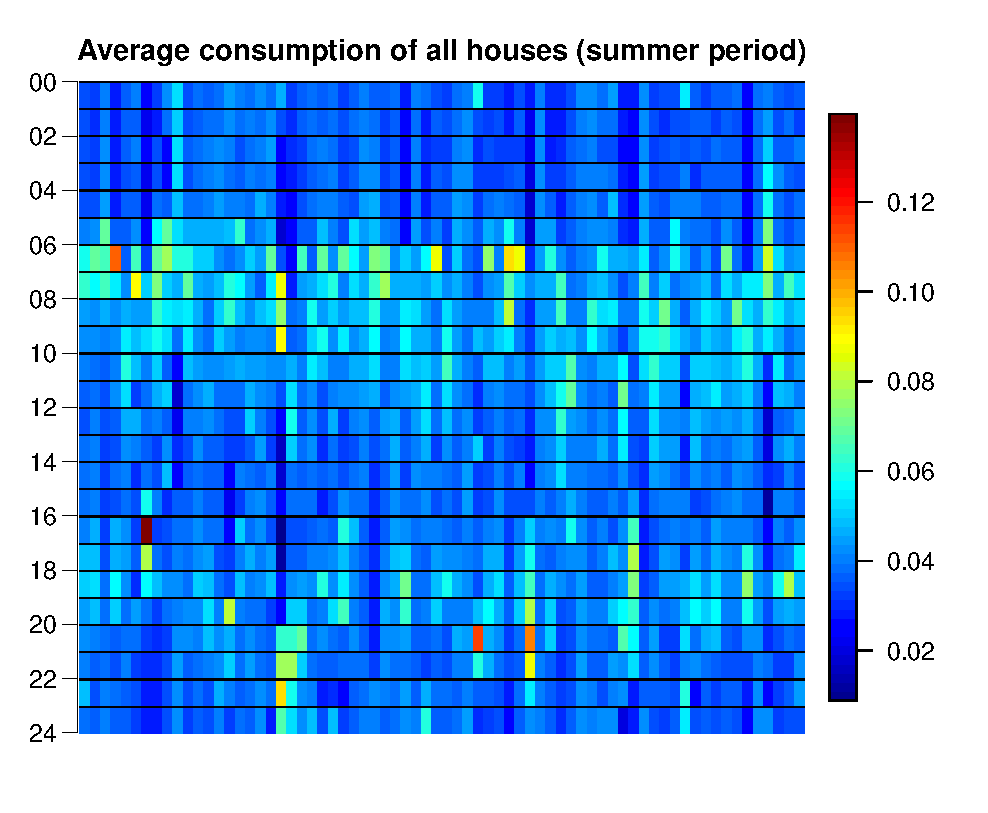
\includegraphics[scale=0.80]{../../../figures/Heatmap_summer.eps}
    \captionof{figure}{The normalized average consumption of every house during the day in the summer period. This is characterized by the days where the average outside temperature is above 15 degrees. The horizontal lines indicate the hours and each vertical strip is a house. The scale indicates the fraction of the total consumption during the day \label{fig: Hourcons_summer}.}
\end{figure}

\begin{figure}[H]
    \centering
    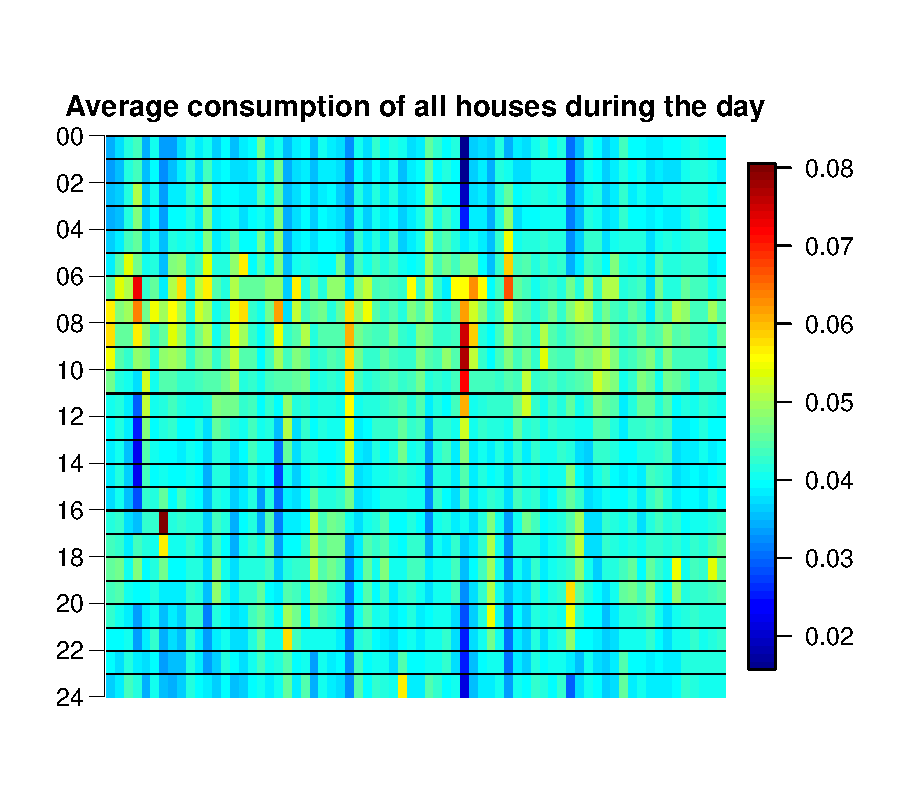
\includegraphics[scale=0.80]{../../../figures/Heatmap_winter.eps}
    \captionof{figure}{This figure shows the same as \cref{fig: daily_cons}, but only for the winter period, characterized by an outside temperature below 12 degrees
    \label{fig: Hourcons_winter}.}
\end{figure}

\section{Description of the Hourly Consumption}
\noindent \cref{fig: Hourcons_summer} and \cref{fig: Hourcons_winter} show the average consumption of each house during the day for the summer period and the winter period respectively. The different hours can be seen on the $y$-axis, and the colour coding show the fraction of that house's consumption in that hour interval. Each vertical strip of colours is a single house and each strip sums up to $1$. Looking at the summer period in \cref{fig: Hourcons_summer}, a generel trend is apparent. The consumption is usually larger around $7$ AM and to some degree around $7$ PM. Almost every house peaks in one of these periods, and some peaks go up to $12\%$ of the daily consumption. On the other hand, there is almost no consumption between $11$ PM and $5$ AM. The same goes for the afternoon between $1$ PM and $4$ PM. \cref{fig:HourDistribution} shows the average distribution of all houses together with lines indicating the quantiles. On the figure it can be seen that the intervals $06-11$ AM and $06-07$ PM are in the top quantile. The periods $00-05$ AM and $03-04$ PM are where the consumption is lowest.

\noindent These trends make sense. In the summer period, not much energy is used for heating the house. There is usually a significant amount of tap water consumption in the morning, when people take warm baths and make breakfast. Sometimes a dishwasher might be running as well. Then there is not much consumption while people are at work or in school. When they get home in the late afternoon the consumption rises again, as they prepare for dinner or use hot water in other ways. During the night time the consumption becomes low again.



\noindent The winter period shown in \cref{fig: Hourcons_winter} is a bit different. There are still significant peaks in the morning, and to some extent in the evening as well, but in general the consumption is more spread out on the entire day. This is mostly because of the heating consumption in the winter period. While people are not at home or while they are sleeping, the heating is still turned on. The highest peaks only go to $8\%$ of the daily consumption here. One house stands out in this plot. A bit to the left of the middle there is a house where the consumption is several times higher between $8$ AM and $12$ noon. This house has almost no consumption during the night. But the house is not a commercial building and its area is only 138 $m^2$. So this house appears to have an efficient night time drop for their thermostat.


\noindent These figures illustrate the general trend of the houses, but it is hard to compare them in a meaningful way. \cref{fig: Season_dist} shows the average distribution of all houses during the day and both the winter period and the summer period show the same trends that was discussed above. But this plot also shows how the winter period is more smoothed out than the summer period. Keep in mind that the lines only show the relative distribution, and they do not take into account that the consumption in the average winter period is significantly higher. As one can see on the y-axis, the difference between the two curves is very small. A night time period can be defined as the hours $23-05$. This is the period after the consumption drops in the evening, and before it rises in the morning. In this period, the houses on average use $21.9\%$ of their daily consumption in the summer period, and $23.7\%$ in the winter period. A completely uniform consumption would be $25\%$. It is not surprising that the consumption in the night hours is lower than the average. Neither is it surprising that the consumption at night in the summer period is relatively lower than in the winter period. The extra cost of heating the house makes the consumption more spread out on the 24 hours of the day. But it is surprising that the difference between the summer period and the winter period is only $1.8$ percentage points. With this in mind, the time series modelling will now be introduced.


\begin{figure}
    \centering
    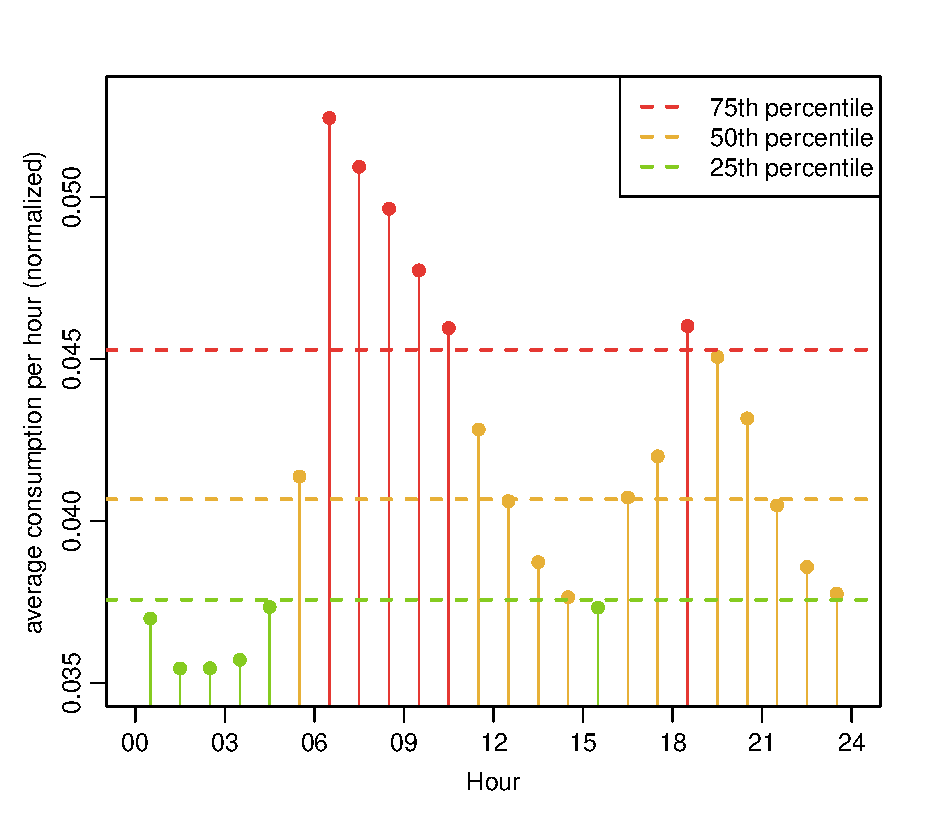
\includegraphics[width=0.8\textwidth]{../../../figures/HourDistribution.eps}
    \caption{The average consumption of all houses during the day. Each point indicate the average consumption in the previous hour interval. The hours in the 75th percentile are $06-11$ AM and $06-07$ PM.}
    \label{fig:HourDistribution}
\end{figure}

\begin{figure}
    \centering
    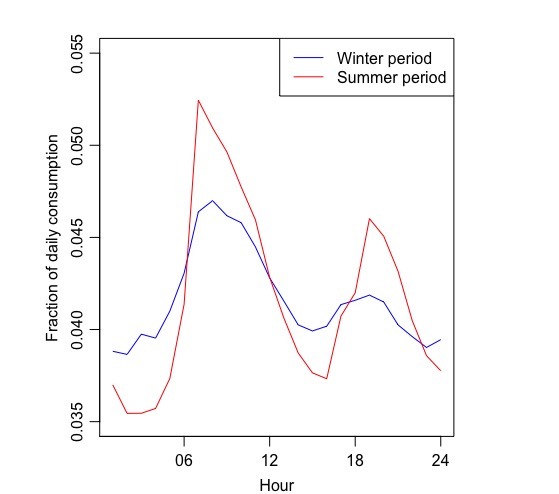
\includegraphics[width=0.7\textwidth]{../../../figures/Season_distribution.jpeg}
    \caption{The average distribution of the heat consumption during the day for the winter period and the summer period respectively. The winter period is more smoothed out, but they are very similar.}
    \label{fig: Season_dist}
\end{figure}


\section{The ARMA Models and Their Extensions}
The consumption of a house during a certain period with hour intervals is a time series. A time series is a realization of a stochastic process. In this section the ARMA model will be introduced, and an extended ARMA model, the ARIMAX model, will be fitted to the consumption. The theory of the ARMA model is based on chapter 5 from the book "Time Series Analysis" by Henrik Madsen \cite{Time_Series_Analysis}. The ARMA model fits the data to a linear stochastic process, with an autoregression part (AR) and a moving average part (MA). A linear process $\{Y_t\}$ is a process that can be written as
\begin{equation}
    Y_t - \mu = \sum_{i=0}^{\infty} \psi_i \varepsilon_{t-i}, \label{linearProcess}
\end{equation}
where $\mu$ is the mean of the process, $\{\varepsilon_i\}$ is white noise and $\{\psi_i\}$ is the weights. For now, the mean $\mu$ is assumed to be zero. To define the ARMA model, the backwards shift operator $B$ is first introduced as $BY_t = Y_{t-1}$. An ARMA process has the form
\begin{equation}
    \phi (B)Y_t = \theta (B) \varepsilon_t,
\end{equation}
where $\phi$ and $\theta$ are polynomials on the shift operator $B$ with degree $p$ and $q$ respectively. $\theta(B)$ is the autoregressive part and $\phi(B)$ is the moving average part. The process is denoted as an $ARMA(p,q)$ process. ARMA processes are linear. If one applies $\psi(B)$ to $Y_t$ and substitutes $Y_{t-1}$, then $Y_{t-2}$ and so forth, the form in \cref{linearProcess} is obtained.

\noindent An ARMA process is stationary if all the roots of $\phi(z^{-1})$ are within the unit circle. Stationarity is a very desirable property. In a stationary process, the mean and variance does not change over time, but often processes will not be stationary due to long term trends. For example the mean consumption of a house has a periodic trend during the year. This was clearly illustrated in \cref{fig: daily_cons}. But long term trends can be eliminated by introducing differencing. Instead of modelling the process $\{Y_t\}$, one can model the process $\{Y_t - Y_{t-1}\}$, i.e. the difference between observations. This is formalized with the difference operator $\Delta = (1-B)$. The differenced ARMA model is called the $ARIMA(p,d,q)$ model, or the autoregressive \textit{integrated} moving average model. It has the form
\begin{equation}
    \phi (B) \Delta^d Y_t = \theta (B) \varepsilon_t,
    \label{ARIMA}
\end{equation}
where $d\in \mathbb{N}$ is the differencing factor. Apart from the long term trends, the model might also have short term periodic trends. In this case a 24 hour periodic trend would be expected. The ARIMA model can be expanded to a seasonal ARIMA with season $s$, such that
\begin{equation}
    \phi (B) \Phi (B^s) \Delta^d \Delta_s^D Y_t = \theta (B) \Theta (B^s) \varepsilon_t.
    \label{eq:ARIMA}
\end{equation}
This is a seasonal $ARIMA(p,d,q)\times (P,D,Q)_s$. $\phi$, $B$, $\Delta$ and $\theta$ are defined as in \cref{ARIMA}. But here $\Phi$ and $\Theta$ are also included. They are polynomials in $B^s$ of degree $P$ and $Q$ respectively. The differencing factor of the seasonal component of the model is denoted $D$.

\noindent In this particular project there is access to the consumption, but also to the weather data. The temperature is also a time series, and it can be used as input to the ARIMA model to make a better fit. This is called using an exogenous variable. When an exogenous variable is used, the model is called an ARIMAX model. The following part is based on Chapter $8$ in \cite{Time_Series_Analysis} and the \texttt{R} documentation of \texttt{arima}. The model looks like this
\begin{equation}
    \phi (B) \Phi (B^s) \Delta^d \Delta_s^D Y_t = \theta (B) \Theta (B^s) \varepsilon_t + \omega(B) X_t,
    \label{eq:ARIMAX}
\end{equation}
where $X_t$ is the exogenous variable and $\omega(B)$ is a polynomial in $B$. The exogenous part can also be differenced or have seasonal components, but in this project those extensions will not be explored. In fact only $\omega(B)=\omega_0$ will be used in the modelling process. The \texttt{arima} function used for the ARIMAX processes does not estimate the exogenous parameters according to Equation \cref{eq:ARIMAX}. It actually starts out by making a regression of the series $\{Y_t\}$ on the exogenous variable $\{X_t\}$. Then this fit is substituted for $Y_t$ in Equation \cref{eq:ARIMA}. This approach is less precise, since it executes the parameter estimation in two steps, first for the exogenuous variable, then for the rest of the variables. An alternative method is to use the \texttt{marima} package in \texttt{R}. This package computes the estimates in Equation \cref{eq:ARIMAX} by using different approximation methods than the \texttt{arima} function. Neither methods should be considered "correct", but they produce different results.

\section{Applying the Models}
In this section, different ARIMAX models will be applied to the data. Transformations are not applied to the data, because the results should be as easy to interpret as possible. First the \texttt{arima} function in \texttt{R} will be used to test different models. The models will include a season of 24 hours. The \texttt{arima} models will then be used to make predictions on data not used for training, to see how well the ARIMAX model performs in general on the data set. Examples will be given on how such predictions could be visualized in WATTS. After that, new models will be generated using the \texttt{marima} package in \texttt{R}. These models will be used to calculate the step response of the temperature, which can be compared to the temperature estimates in the linear regression models. To apply time series models, the data has to be complete without gaps. For this reason the entire data set is used, not only the winter period. Two weeks in january 2019 are left out for testing. The temperature used in the models will be the altered temperature defined by
\begin{equation}
    T_{winter} = \begin{cases}
        \alpha - T & \text{if } T\leq \alpha\\
        0 & \text{Otherwise}
    \end{cases},
    \label{eq:Ttilde_hour}
\end{equation}
just as in the models on the daily data.

\subsection{Modelling with the ARIMA Function}
To generate a model, one must decide a model order. It is important that the model is not too complex. With the amount of data available for each house, too many parameters in the model causes the running time to increase drastically. More importantly, sometimes the optimization method used in the $arima$ function does not converge. This happens more often when there are more parameters, and the model should be applicaple to as many different houses as possible. As mentioned in the section above, stationarity is an important property. If the order of the autoregressive part (both non-seasonal and seasonal) is too high, the model will not be stationary unless differencing is used. Differencing on the other hand makes the model more obscure and harder to interpret. If the model is only differenced once, it means that it models the difference between one hour and the one before that. If the seasonal part is differenced, it models the difference between an hour and the same hour the day before.

\noindent These considerations have led to the conclusion that a $(1,0,1)\times (1,0,1)$ model is a good starting point. Written in the form of \cref{eq:ARIMA} it is
\begin{equation}
    (1-\phi_1 B)(1-\Phi_1 B^{24})X_t = (1+\theta_1 B)(1+\Theta_1 B^{24}) \varepsilon_t. \label{eq:model1}
\end{equation}
Here $Y_t$ is substituted with the regression fit $X_t = Y_t -\beta T'_t$. As mentioned earlier \texttt{arima} first estimates the regression variable $\beta$, before inserting $X_t$ into the model. The negative sign of the $\phi$ values is due to the convention of the \texttt{arima} function, where $Y_t$ is isolated to one side of the equation. The model can also be formulated as
\begin{align}
    X_t = &\phi_1 X_{t-1} + \Phi_1 X_{t-24} + \phi_1 \cdot \Phi_1  X_{t-25}\nonumber\\  &+ \theta_1 \varepsilon_{t-1} + \Theta_1 \varepsilon_{t-24} + \theta_1 \cdot \Theta_1 \cdot \varepsilon_{t-25} + \varepsilon_t.
\end{align}

\noindent For most houses this model is not stationary and the optimization does not converge. \cref{fig:Model1_stationarity} shows the roots of the model when applied to house 55. On the left the AR roots are illustrated, on the right the MA roots are illustrated. When considering stationarity, only the AR roots are of interest. Here it can be seen how every inverse AR root is on the edge of the unit circle. This model introduces $25$ roots in $\phi$, $1$ from the non-seasonal part, and $24$ from the seasonal part. \cref{fig:Model1_stationarity18} shows the same for house 18, where every AR root is on the edge of the unit circle except for one. As many of the inverses of these roots as possible should be inside the unit circle. This is not as important if the AR parameters are not very significant. But for this model, the parameters are very significant for both seasonal and nonseasonal AR, and for both house 55 and 18. The values are listed in \cref{tab:model1_param55} and \cref{tab:model1_param18} in the appendix. The AR components are significant for most of the houses. For this reason, it makes the most sense to difference the the model, and since the seasonal AR produces the most roots, the seasonal part will be differenced. The one root from the non-seasonal part might still be on the edge of the unit circle, but the rest will most likely not be.



\begin{figure}
    \centering
    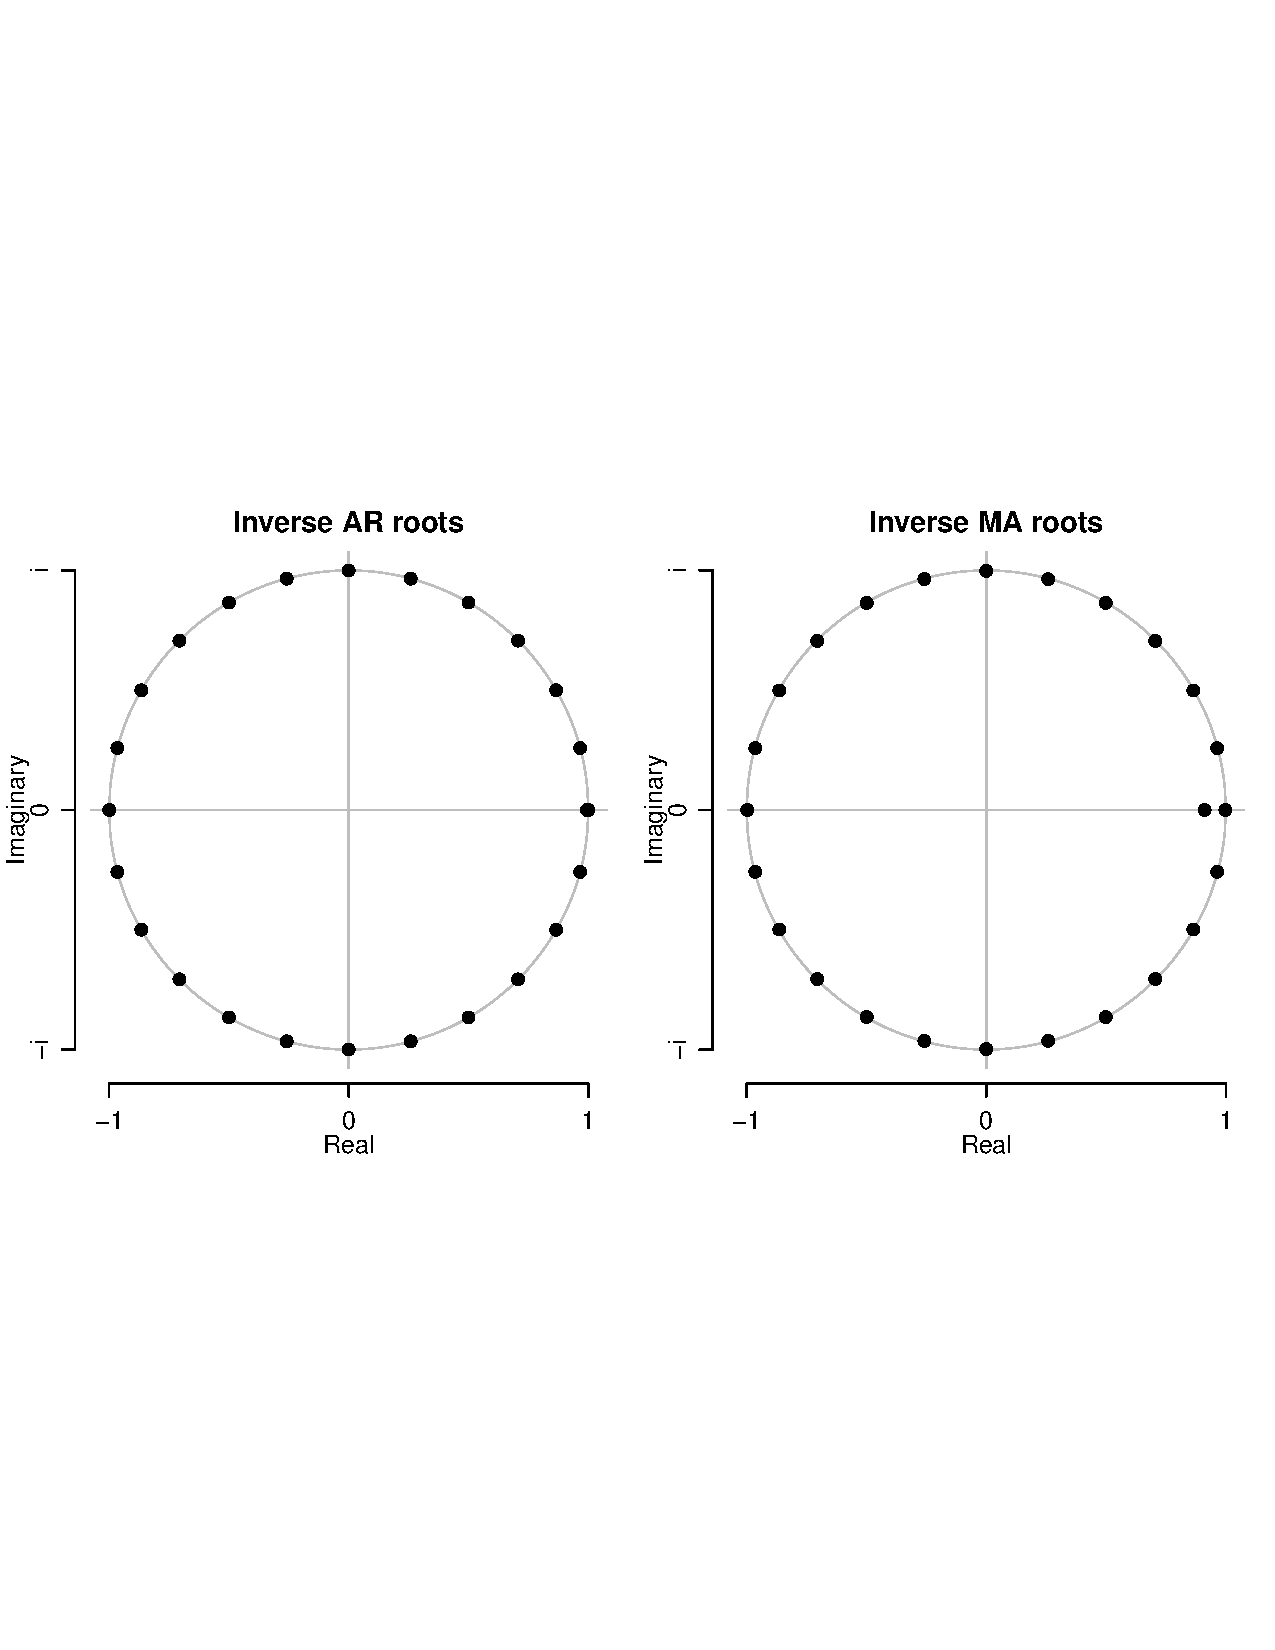
\includegraphics[width=0.8\textwidth]{../../../figures/arimax/Stationarity_model1.pdf}
    \caption{The roots of the first model when applied to house 55. All the inverse AR roots are on the edge of the unit circle}
    \label{fig:Model1_stationarity}
\end{figure}

\begin{figure}
    \centering
    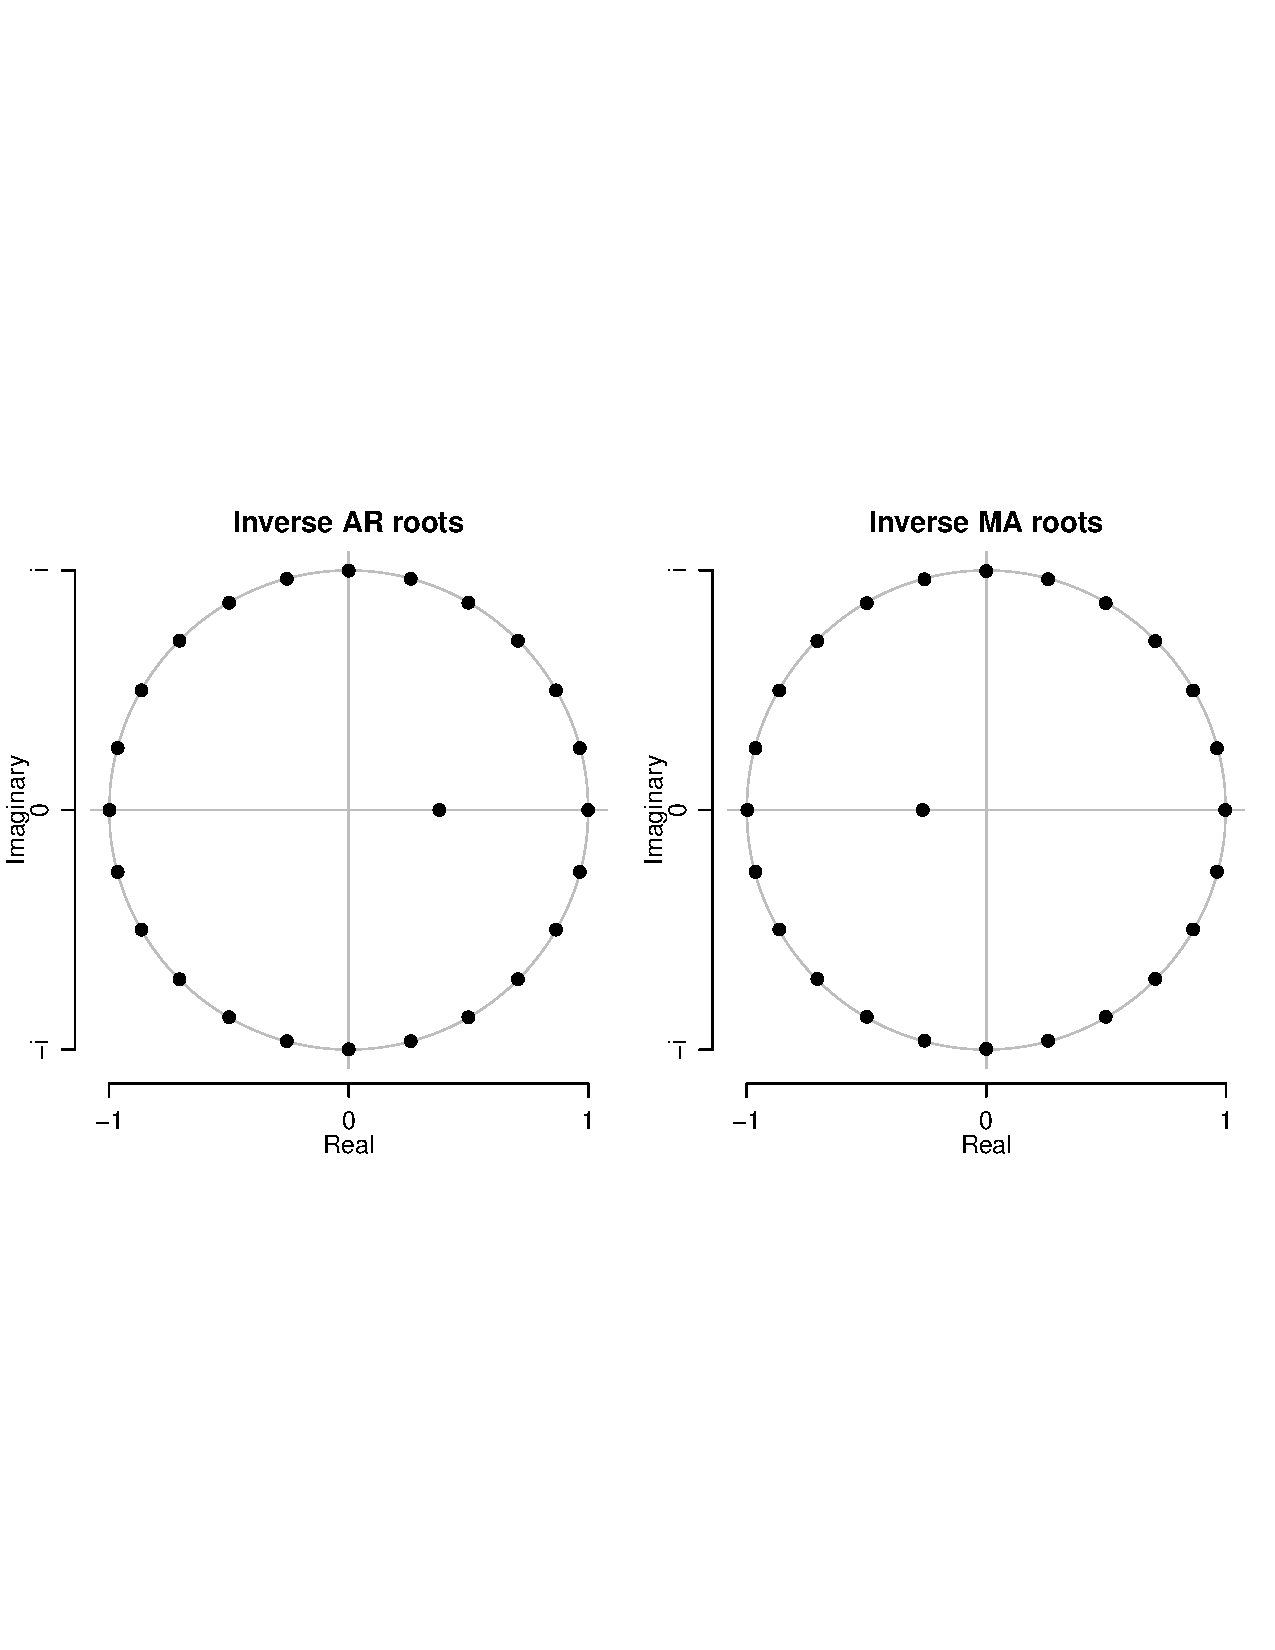
\includegraphics[width=0.8\textwidth]{../../../figures/arimax/Stationarity_model1_18.pdf}
    \caption{The roots of the first model when applied to house 18. All the inverse AR roots are on the edge of the unit circle except for one}
    \label{fig:Model1_stationarity18}
\end{figure}


\noindent Thus, the next model is a $(1,0,1)\times(1,1,1)$ model, written as
\begin{equation}
    (1-\phi_1 B)(1-\Phi_1 B^{24})(1-B^{24})X_t = (1+\theta_1 B)(1+\Theta_1 B^{24}) \varepsilon_t.
\end{equation}
This is the same model as in \cref{eq:model1}, except for the differencing. When rewritten, the model becomes:
\begin{align}
    X_t-X_{t-24} = &\phi_1 (X_{t-1}-X_{t-25}) + \Phi_1 (X_{t-24}-X_{t-48}) + \phi_1 \cdot \Phi_1  (X_{t-25}-X_{t-49})\nonumber  \\  &+ \theta_1 \varepsilon_{t-1} + \Theta_1 \varepsilon_{t-24} + \theta_1 \cdot \Theta_1 \cdot \varepsilon_{t-25} + \varepsilon_t. \label{model101111}
\end{align}
This shows clearly how the model now operates on the difference between a value and the same value a day earlier. Firstly, the stationarity of this model should be evaluated. The inverse roots of house 55 and 18 are shown in \cref{fig:Model2_stationarity55} and \cref{fig:Model2_stationarity18} respectively. For house 55 the 24 seasonal AR roots are within the unit circle. The last root is not. While this is not optimal, it is definitely better than the last model without differencing. For house 18 all the roots are sufficiently within the unit circle. This is true for most of the houses the model was applied to. So in terms of stationarity the model performs well over all. It would be better to introduce non-seasonal differencing as well, but to keep the model simple no further differencing is applied.


\begin{figure}
    \centering
    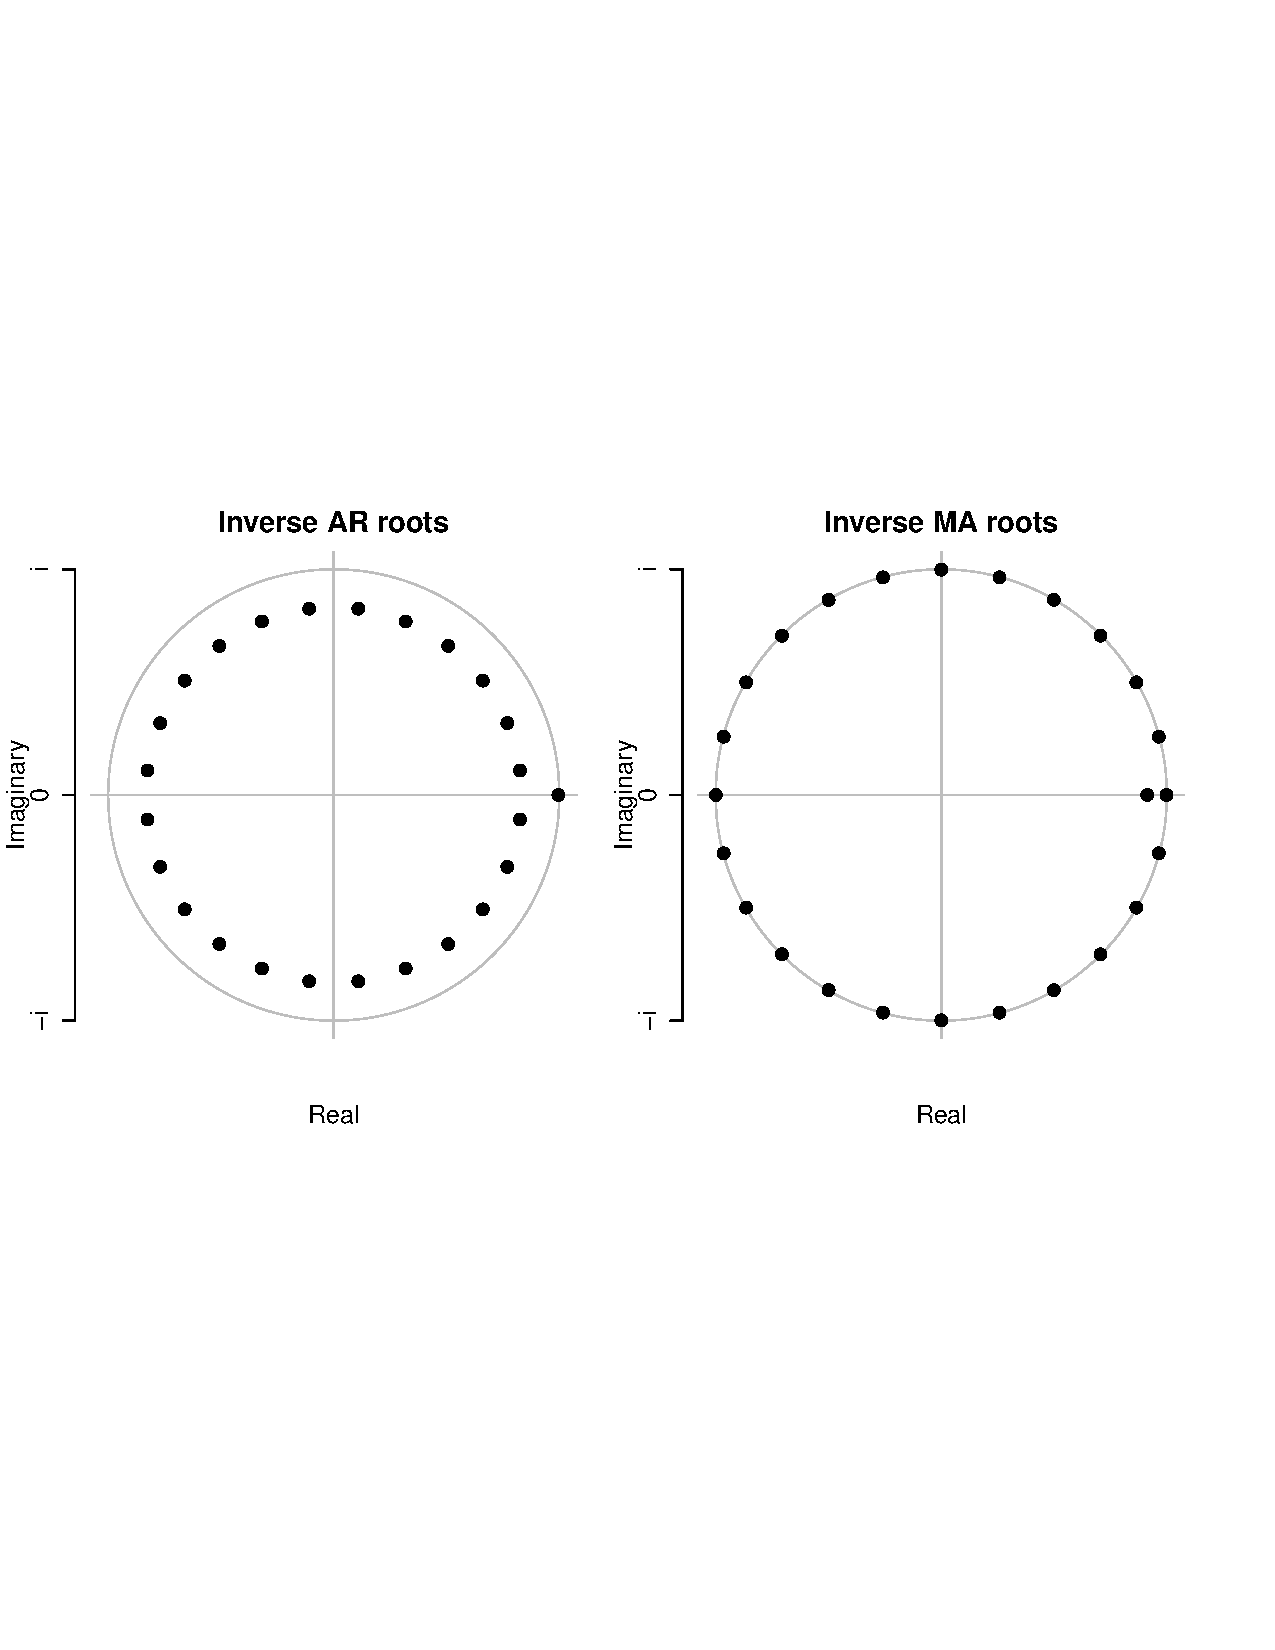
\includegraphics[width=0.8\textwidth]{../../../figures/arimax/Roots_55.pdf}
    \caption{The roots of the second model when applied to house 55.}
    \label{fig:Model2_stationarity55}
\end{figure}


\begin{figure}
    \centering
    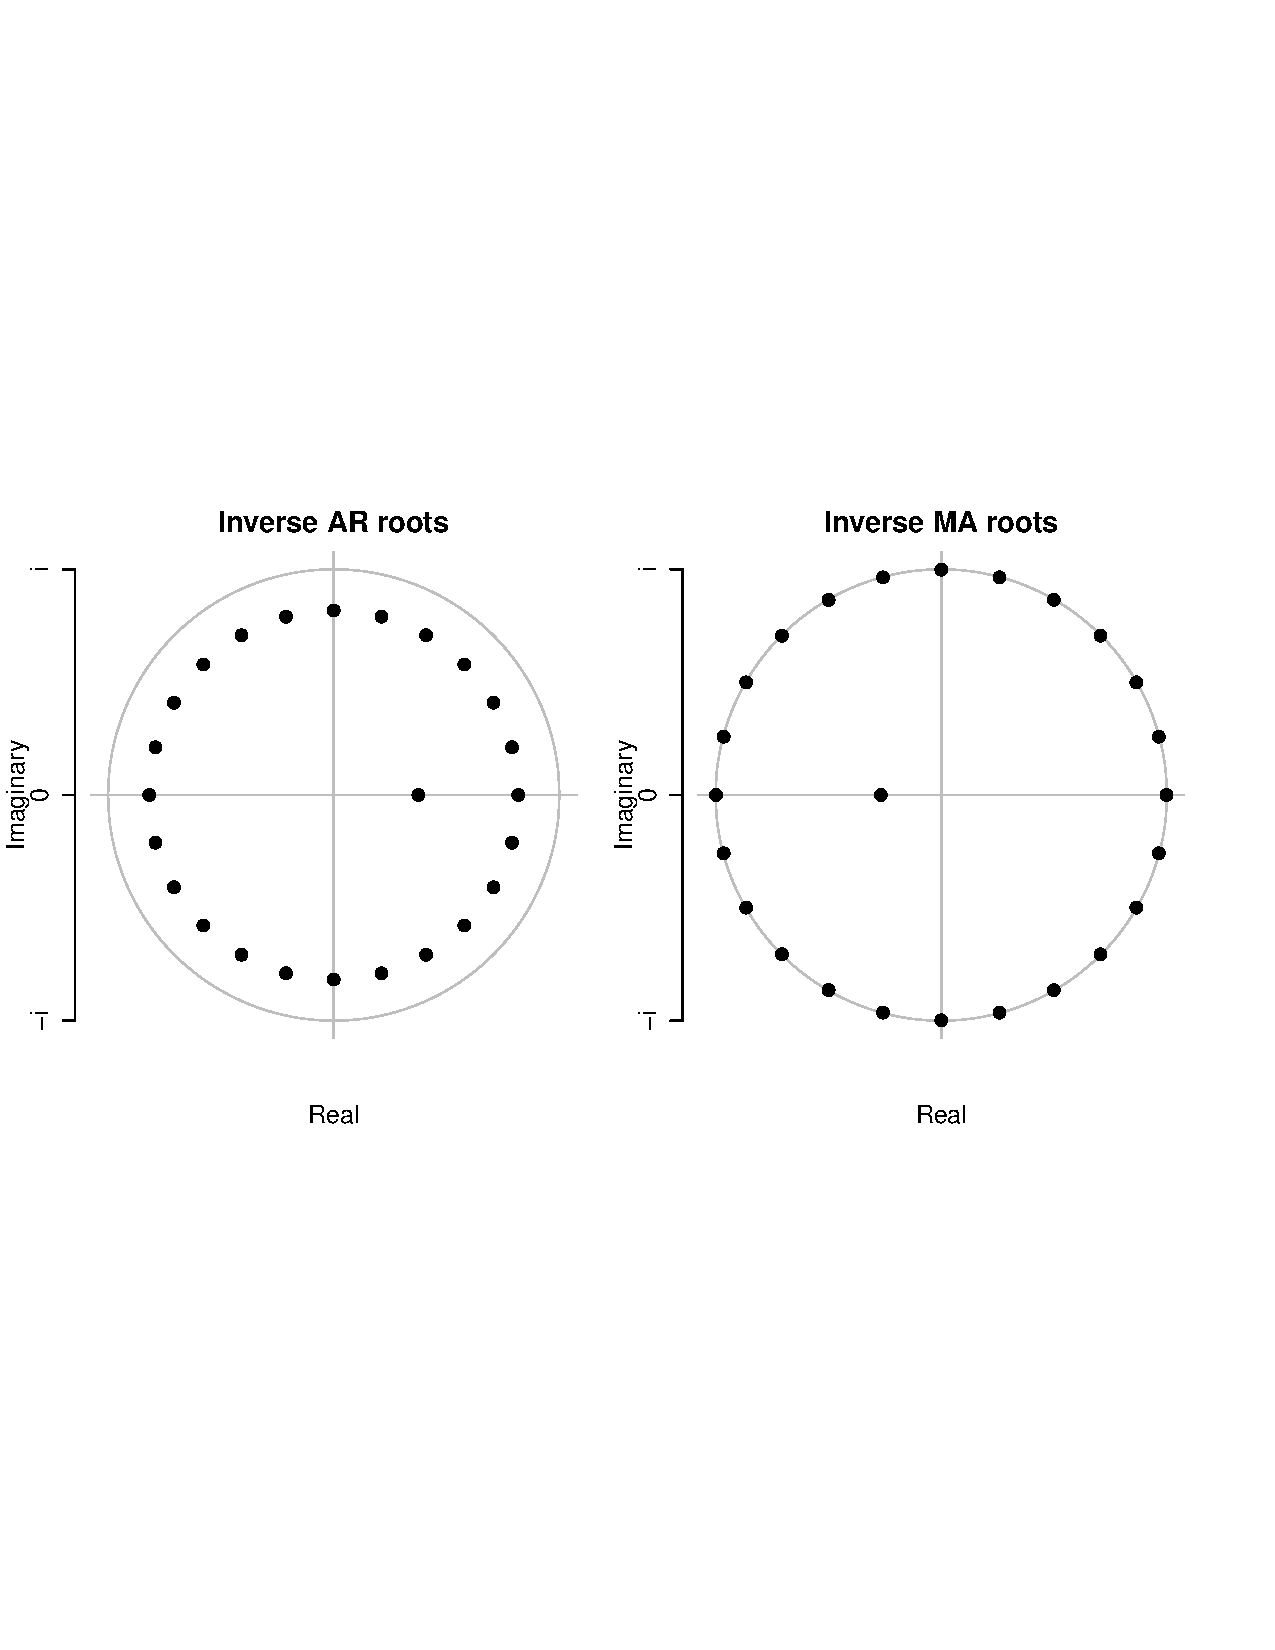
\includegraphics[width=0.8\textwidth]{../../../figures/arimax/Roots_18.pdf}
    \caption{The roots of the second model when applied to house 18.}
    \label{fig:Model2_stationarity18}
\end{figure}

\noindent After considering the stationarity of the model, the significance of the parameters is examined. The model is applied to $70$ houses, making it hard to evaluate based on a few houses. \cref{tab:ParamSig_Model1} gives an overview of how many models have significant parameters. It shows how many of the houses have parameters below two and three standard deviations respectively. It can be seen that the seasonal AR1 is the parameter that is most often not significant. For $36$ of the houses the parameter value is below two standard deviations, which is about half of the houses. For $50$ of the houses, the parameter is below three standard deviations, so most of them are not significant, or barely significant. Looking specifically at house 55, the parameter values and standard deviations are listed in \cref{tab:ParamSig_House55}. Here the seasonal AR is only just a little bit bigger than the standard deviation, making it insignificant. If the estimates were inserted into \cref{model101111}, one would get the equation
\begin{align}
    X_t-X_{t-24} =& 0.9949 (X_{t-1}-Y_{t-25}) - 0.0122 (X_{t-24}-X_{t-48}) \nonumber\\  & - 0.0121  (X_{t-25}-X_{t-49}) - 0.9124 \varepsilon_{t-1} \nonumber\\
    &-0.9572 \varepsilon_{t-24} + 0.8733 \varepsilon_{t-25} + \varepsilon_t,
\end{align}
for $X_t = Y_t - 0.288 T'_T$. The autocorrelation function (acf) and the partial autocorrelation function (pacf) for this model is visualized in \cref{fig:Model2_acf_55}. There are clearly some significant spikes on the first couple of lags, both in the acf and in the pacf. There are also a few significant lags scattered out on the rest of the function. It should also be noted that the lags around the seasons, indicated by the red lines, do not stand out. The model clearly has problems in the first couple of lags, where there is autocorrelation between the residuals. On the other hand the seasons seem to be accounted for. The rest of the significant lags are relatively random and not very significant. They could be regarded as white noise. The pacf show signs of some oscilleration, but it might just be some distortion in the model. To get a view of the long term effects, \cref{fig:Model2_acf_55_long} in the appendix show the acf and the pacf for an entire week. Here it is still clear that the model is far from perfect, but the biggest issue is the first couple of lags. After that, none of the lags reach more than about $0.05$, which is acceptable. One lag of particular interest is the one at the last red line. This is lag $168$ (the seventh season), which is the autocorrelation between weeks. It shows the autocorrelation between the current residual and the same residual one week earlier. A high autocorrelation in lag $168$ could be a threat to the performance of the model. Fortunately, no lags around this season seem to stand out for house $55$. So for this model the effect between weeks, which is not taken into account, does not seem to have much influence. If one were to try to adress the high correlation in the first lags, the non-seasonal part of the model could be expanded with a higher degree of either AR or MA.


\begin{table}[]
    \centering
    \begin{tabular}{l|ccccc}
    \hline
    \textbf{Parameters} & \textbf{AR1} & \textbf{MA1} & \textbf{SAR1} & \textbf{SMA1} & \textbf{Temperature} \\ \hline \hline
    Below 2 sd & 0   & 3   & 36   & 0    & 6           \\
    Below 3 sd & 0   & 3   & 50   & 0    & 14          \\ \hline
    \end{tabular}
    \caption{The number of houses where each parameter is below two standard deviations and three standard deviations respectively. The $(1,0,1)\times (1,1,1)$ model was applied to $70$ houses in total. The average log likelihood of the model is $-6999$}
    \label{tab:ParamSig_Model1}
\end{table}

\begin{table}[]
    \centering
    \begin{tabular}{l|ccccc}
    \hline
    \textbf{House 55} & \textbf{AR1} & \textbf{MA1} & \textbf{SAR1} & \textbf{SMA1} & \textbf{Temperature} \\ \hline \hline
    Estimate           & 0.9949 & -0.9124 & -0.0122 & -0.9572 & 0.0288      \\
    Standard deviation & 0.0013 & 0.0048  & 0.0111  & 0.0043  & 0.0045      \\ \hline
    \end{tabular}
    \caption{The estimates of the parameters for the $(1,0,1)\times (1,1,1)$ model together with their standard deviations for house 55. The log likelihood of the model is $-5791$}
    \label{tab:ParamSig_House55}
 \end{table}

 \begin{figure}
    \centering
    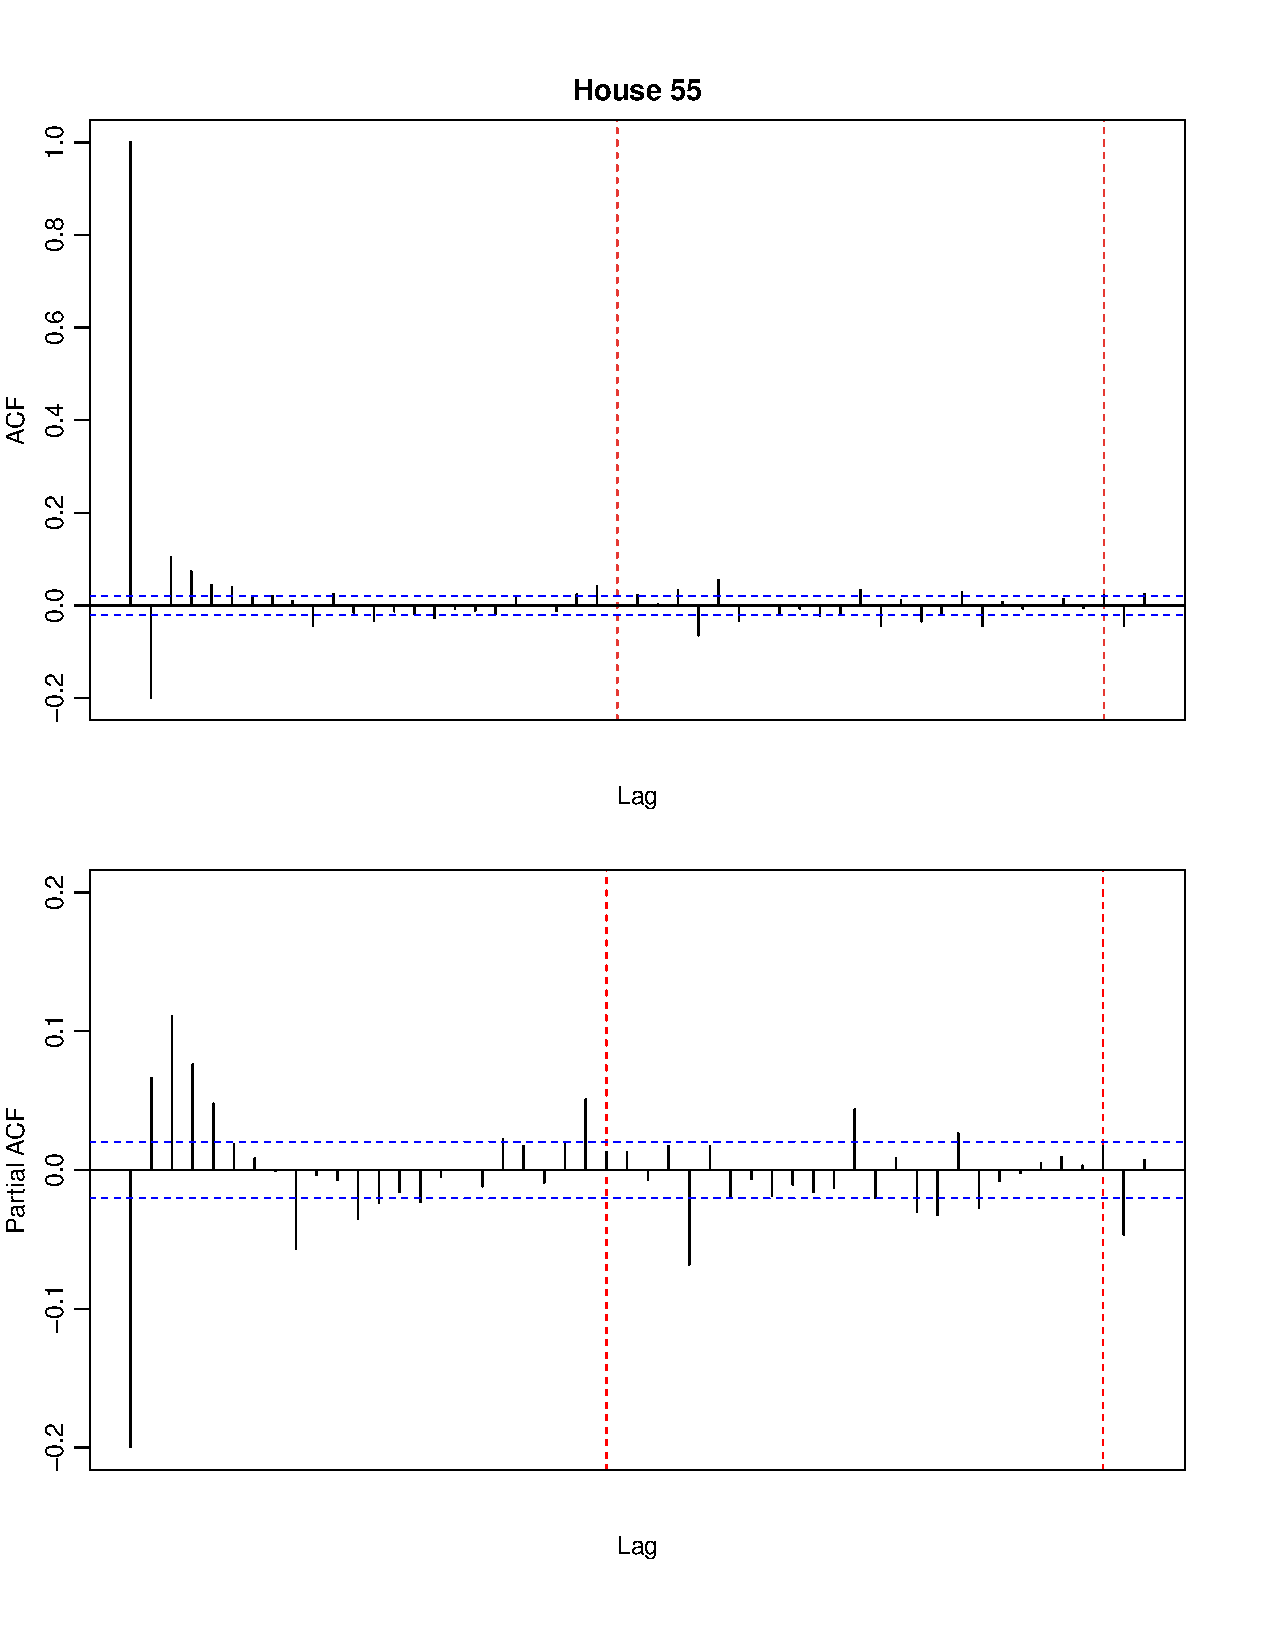
\includegraphics[width=0.8\textwidth]{../../../figures/arimax/ACF_55_short.pdf}
    \caption{The acf and pacf of the second model when applied to house 55. The 24 hour seasons are highlighted with red dashed lines. The blue lines indicate the 95\% confidence interval}
    \label{fig:Model2_acf_55}
\end{figure}


\noindent Now the model will be evaluated for house 18. The estimates for the model are listed in \cref{tab:ParamSig_House18}. Here the seasonal AR1 is even more insignificant than it was for house 55, being less than the standard deviation. The log likelihood of the model for this house $(-12780)$ is also much lower than for house 55 $(-5791)$, or than the average of the model $(-6999)$. After insertion into \cref{model101111} the model for house 18 is
\begin{align}
    X_t-X_{t-24} = &0.3751 (X_{t-1}-X_{t-25}) + 0.008 (X_{t-24}-X_{t-48}) + 0.003 (X_{t-25}-X_{t-49}) \nonumber\\  &+ 0.2672 \varepsilon_{t-1} - 0.9559 \varepsilon_{t-24} - 0.2554 \varepsilon_{t-25} + \varepsilon_t,
\end{align}
Where $X_t = Y_t - 8.15 T'_t$. Looking at the acf and pacf of this house on \cref{fig:Model2_acf_18}, this house does not have the same high autocorrelation in the first lags. Actually both the acf and the pacf look slightly better for house 18 than they did for house 55, even though house 18 overall has shown unpredictable behavior. There are still significant lags in both the acf and the pacf, but as for house 55, they are not very large and can to some extent be regarded white noise. As for the 24 hour seasons, there are no significant outliers. There is no pattern indicating that the residuals for the 24 hour seasons are not sufficiently accounted for in the model. When looking at \cref{fig:Model2_acf_18_long} in the appendix where an entire week is included, there is a single peak at season four that stands out. But since the other seasons do not show the same behavior, it might as well be a coincidence. Just like for house 55 there is no significant peak at the seventh season. Overall, even though there are many significant peaks in both the acf and the pacf, there is no obvious pattern connected to the seasons or the first lags. And none of the peaks reach a value higher than $0.1$.

 \begin{table}[]
    \centering
    \begin{tabular}{l|ccccc}
    \hline
    \textbf{House 18} & \textbf{AR1} & \textbf{MA1} & \textbf{SAR1} & \textbf{SMA1} & \textbf{Temperature} \\ \hline \hline
    Estimate           & 0.3751 & 0.2672 & 0.008 & -0.9559 & 0.0825      \\
    Standard deviation & 0.0171 & 0.0175 & 0.011 & 0.0040  & 0.0078      \\ \hline
    \end{tabular}
    \caption{The estimates of the parameters for the $(1,0,1)\times (1,1,1)$ model together with their standard deviations for house 18. The log likelihood of the model is $-12780$}
    \label{tab:ParamSig_House18}
    \end{table}


\begin{figure}
    \centering
    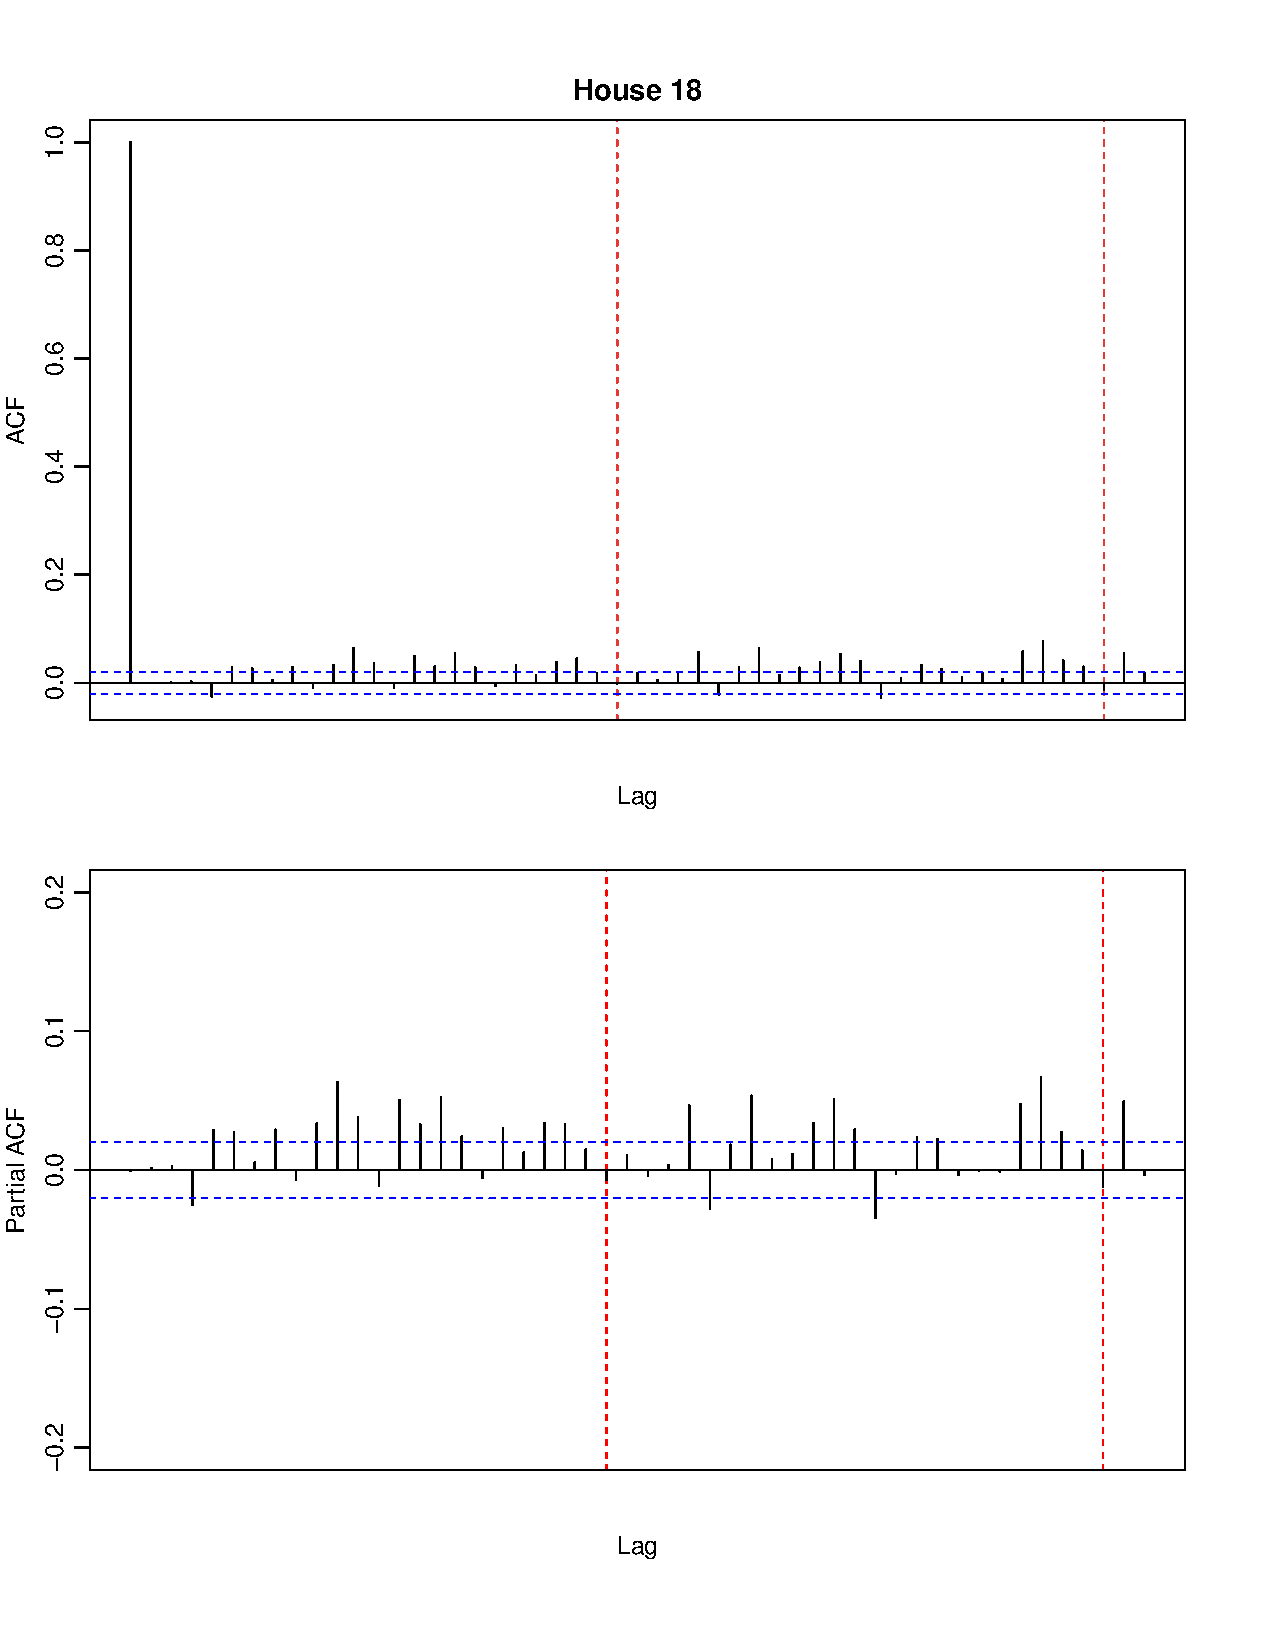
\includegraphics[width=0.8\textwidth]{../../../figures/arimax/ACF_18_short.pdf}
    \caption{The acf and pacf of the second model when applied to house 18. The 24 hour seasons are highlighted with red dashed lines. The blue lines indicate the 95\% confidence interval}
    \label{fig:Model2_acf_18}
\end{figure}


\subsection{Predicting with the ARIMA model}
Now the model found above will be used for predictions. The test data used is two weeks in January 2019. The predictions are made using the \texttt{R} function \texttt{predict}. The  weather data used as input can be seen in \cref{fig:weather_pred_hour}. Just as in the linear regression model, the input series is assumed to be a perfect prediction without measuring errors. The predictions are not one-step predictions, but 14 step predictions. The results of applying the predictions to house 55 can be seen in figure \cref{fig:arima1_pred_55}. It very quickly becomes clear that the data behaves very differently than the model predicts. There are a lot of very high spikes, each followed by an hour with zero consumption. This tendency is not captured at all in the model, and it is clear that the time series models cannot be used for anything useful for this house unless the data is altered in some way. The temperature input was very low for a few days in the end of the test period, but the effect this had on the predictions is minimal compared to the oscillerations in the data. House 18 in figure \cref{fig:arima1_pred_18} shows the same unexpected behavior. There seems to be no connection between the time of day and the massive spikes for either of the houses. And since the spikes are usually followed by a consumption of precisely zero, the behavior seems to be linked to how the data is collected and pre-processed by Aalborg Forsyning. Given that the anomalities come in pairs of measurements that are two or three times higher than the neighbours and than measurements of zero, the most plausible explanation is that several measurements are accidentially grouped into a single hour interval, leaving the next interval with no consumption. The phenomenon with a high spike followed by a zero happens almost every day for most houses, and sometimes several times a day.

\begin{figure}
    \centering
    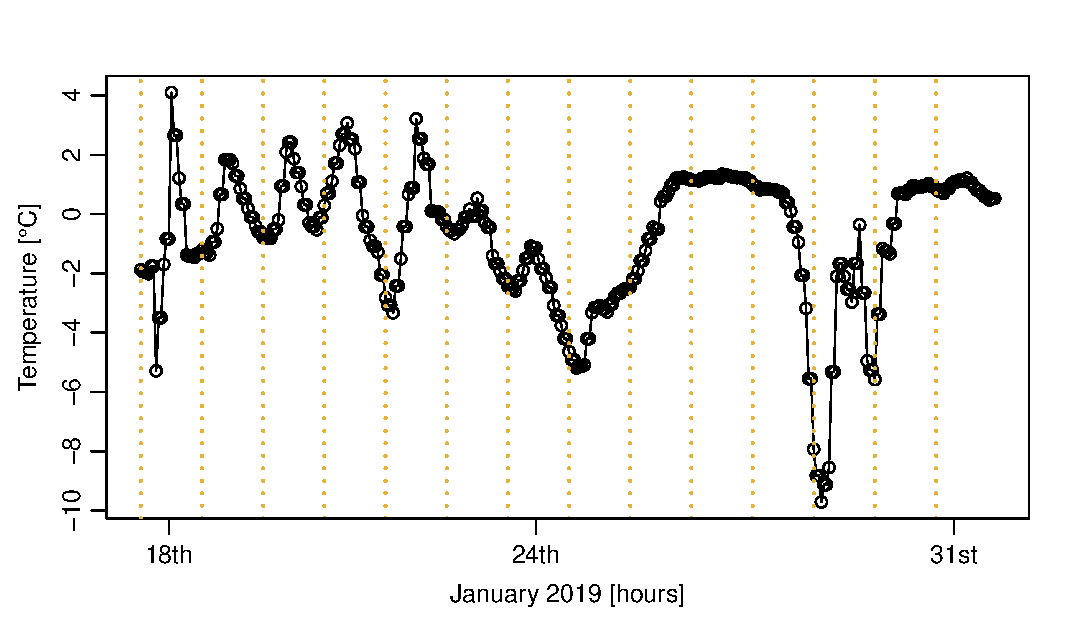
\includegraphics[width=0.8\textwidth]{../../../figures/TestWeatherHour.eps}
    \caption{The input series of the temperature used for predictions made with the arima model}
    \label{fig:weather_pred_hour}
\end{figure}


\begin{figure}
    \centering
    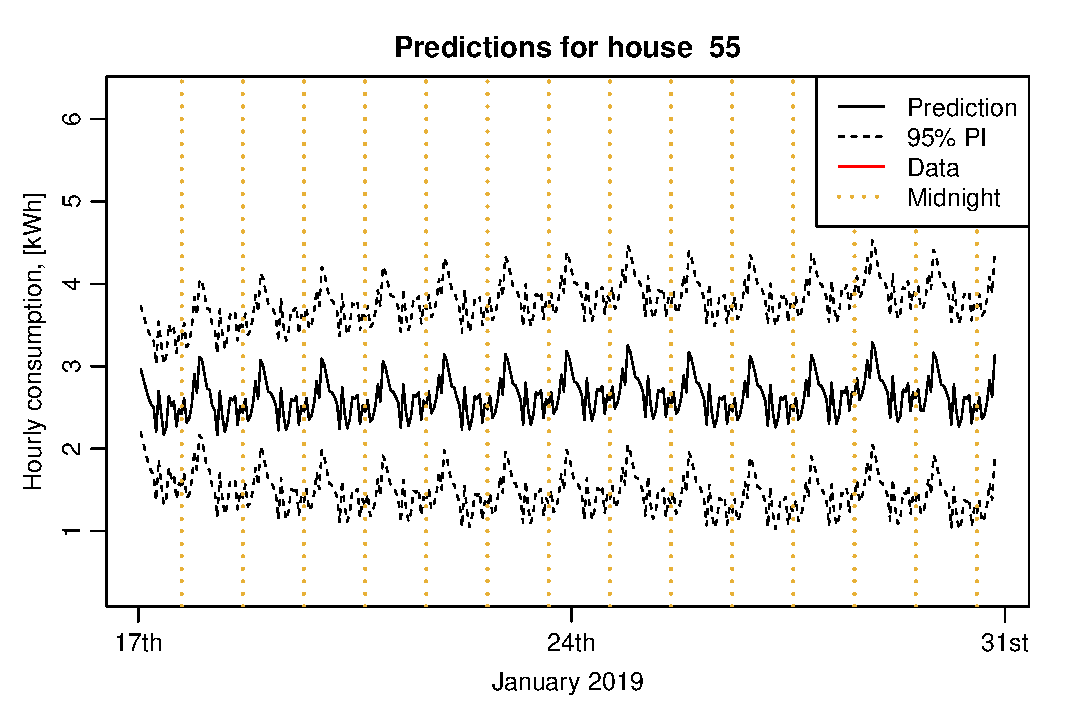
\includegraphics[width=0.8\textwidth]{../../../figures/arimax/arima1_pred_55.eps}
    \caption{Predictions of the arima model for house 55. The data is so far from the predictions and oscillerate so much that the model should not be relied upon}
    \label{fig:arima1_pred_55}
\end{figure}

\begin{figure}
    \centering
    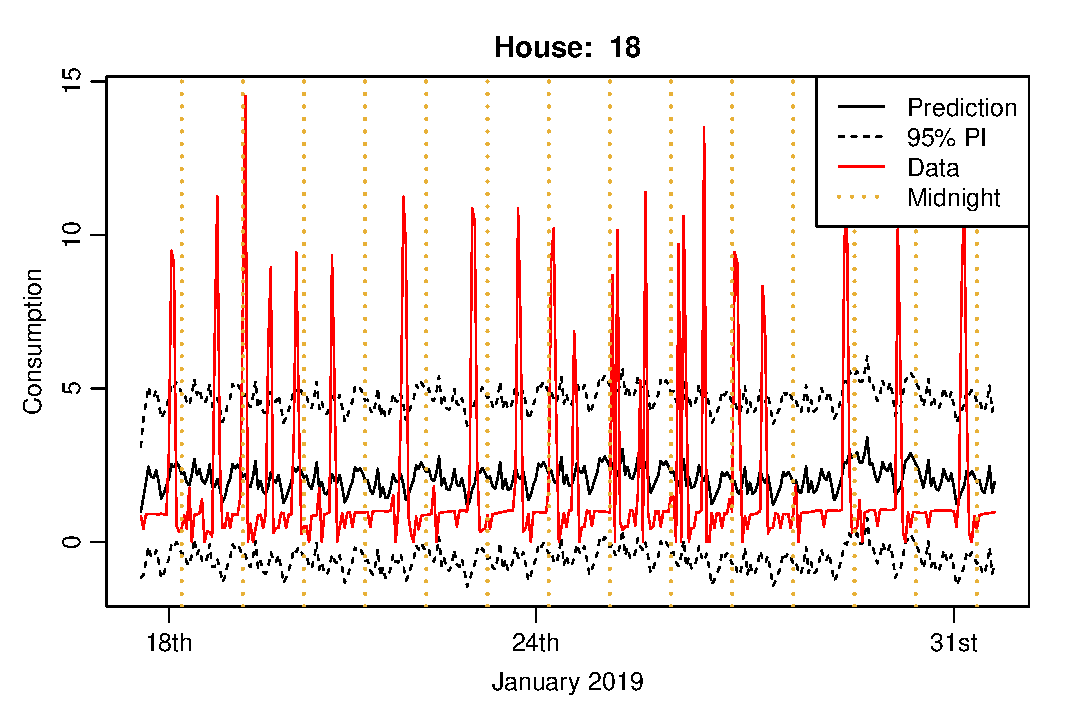
\includegraphics[width=0.8\textwidth]{../../../figures/arimax/arima1_pred_18.eps}
    \caption{Predictions of the arima model for house 18. This is just as bad as for house 18}
    \label{fig:arima1_pred_18}
\end{figure}



\noindent To come up with a more fair evaluation of the model, the data is changed slightly to compensate for the random spikes. Every time there is a consumption of precisely zero, that data point and the one before are both changed to the average of the two. This smoothes out the outliers that seem to be caused by erroneous data collection, without changing the rest of the data too much. The model is now trained and tested on the changed data. The results are shown in \cref{fig:arima1_pred_55} and \cref{fig:arima1_pred_18}. For house 55 the data still have some significant spikes in the first part, but it is more well-behaved in the rest of the test period. Here it is mostly within the prediction interval, but the prediction interval is rather wide. In general the model shows that there is a lot of variance in the data that is not captured by the model. The model could be applied, but it will not perform very well. As for house 18, the data is still way off compared to the predictions. The smoothing did not change the way the data behaved, and there are still a lot of spikes that are so far from the prediction interval, that the model does not say anything useful about this house.


\begin{figure}
    \centering
    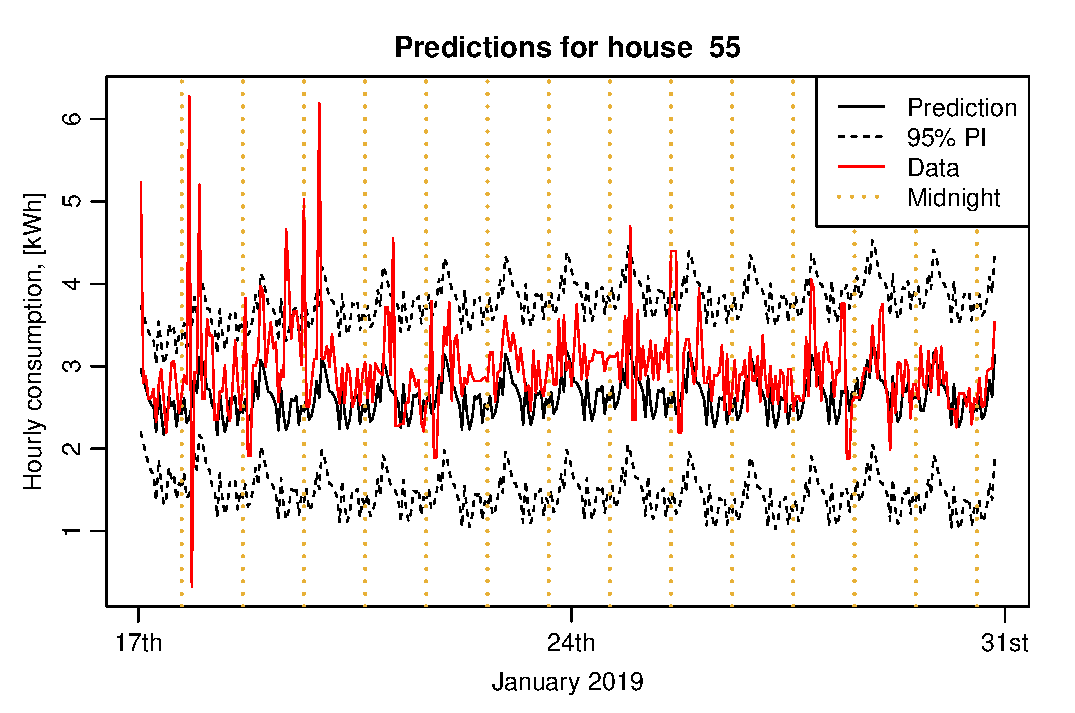
\includegraphics[width=0.8\textwidth]{../../../figures/arimax/arima2_pred_55.eps}
    \caption{Predictions of the arima model for house 55 on the modified data. There are still a few spikes, but the model performs reasonable on this data set}
    \label{fig:arima1_pred_55}
\end{figure}

\begin{figure}
    \centering
    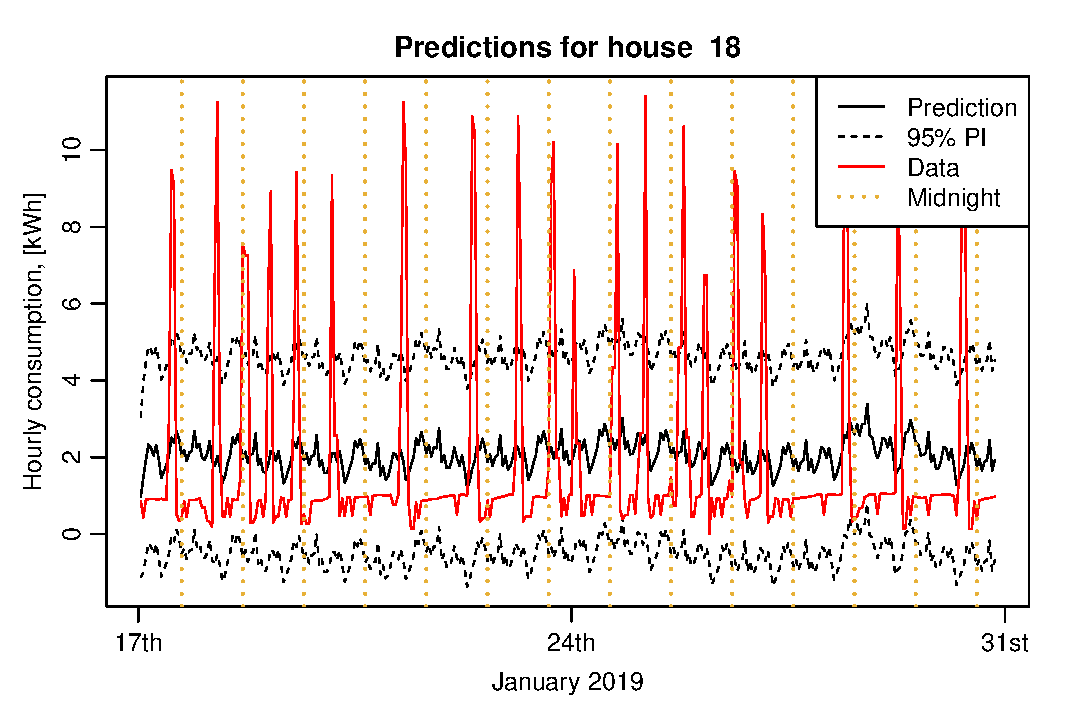
\includegraphics[width=0.8\textwidth]{../../../figures/arimax/arima2_pred_18.eps}
    \caption{Predictions of the arima model for house 18 on the modified data.}
    \label{fig:arima1_pred_18}
\end{figure}


\noindent For the houses that only had data between September 2018 and January 2019, it turned out that there were no anomalities of the type described earlier in this section. This could mean that the data from these houses is collected in a more reliant way. Therefore predictions for one of these houses will also be included. The predictions are illustrated in figure \cref{fig:arima1_pred_6}. The figure shows clearly that the hourly data is still much to unstable to apply the models. There is a lot of variance that is not captured at all in the predictions, and the prediction interval is pretty wide.


\begin{figure}
    \centering
    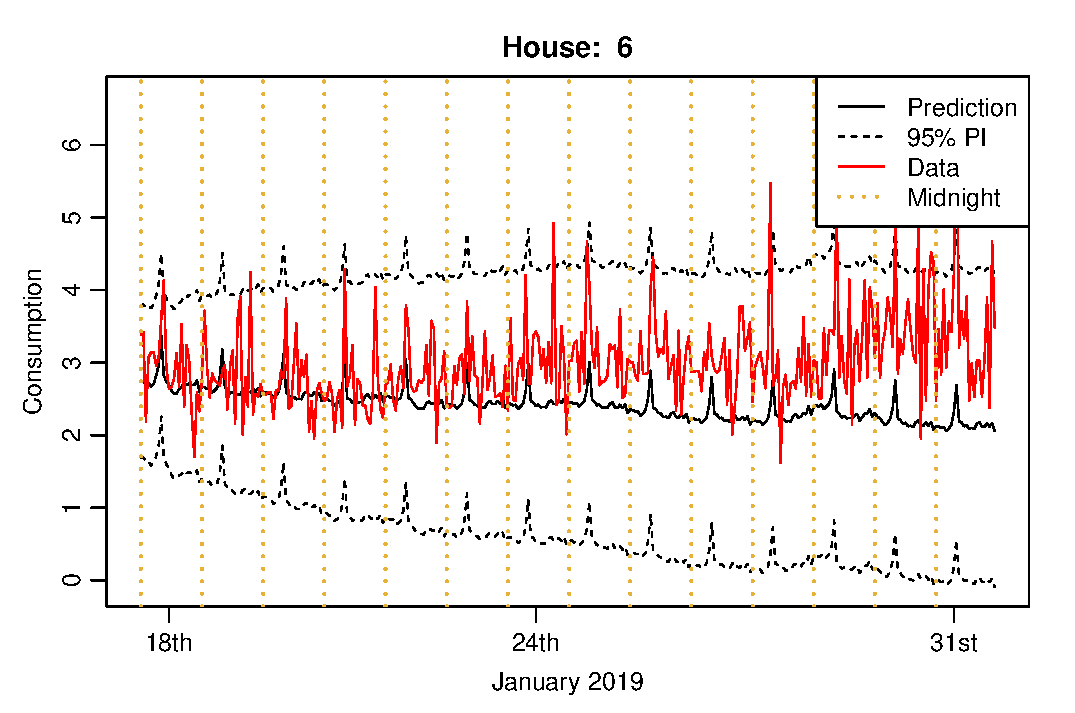
\includegraphics[width=0.8\textwidth]{../../../figures/Pred14days6.eps}
    \caption{Predictions of the arima model for house 6, which is one of the houses with data for a shorter period}
    \label{fig:arima1_pred_6}
\end{figure}



\subsection{Visualization of the results}

\noindent The results recieved from the time series models so far have not been very reliant, and in general the model should not be used for predictions at this stage. But if one were to visualize the predictions found, it could be done by making a colouring similar to that of the regression model. An example is shown in \cref{fig:app6} with predictions for just two days. The colouring is made in the same way as for the predictions made by the regression model in \cref{fig: lmpred_col_55L}, where there according to the model there should be an equal amount of each colour.

\begin{figure}
    \centering
    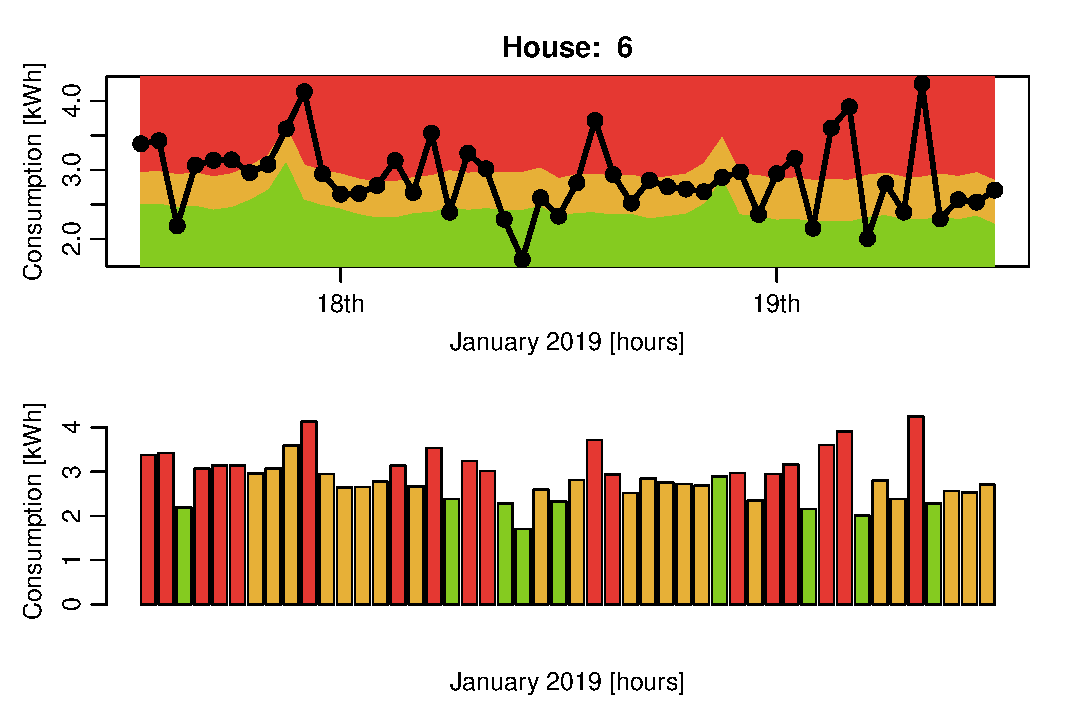
\includegraphics[width=0.8\textwidth]{../../../figures/AppHour6.eps}
    \caption{Visualization of the results of the arima model applied to house 6 for two days in January 2019. The exact period is from $00:00$ on the 18th of January to $23:00$ on the 19th of January}
    \label{fig:app6}
\end{figure}






\subsection{Modelling with the MARIMA Function}
It has been mentioned in Section 5.2 that MARIMA works in a fundamentally different way than the ARIMA function. It uses an iterative method to estimate the parameters, including all the regression variables. The exact procedure can be seen in \cite{marima}. The goal is to make a model that can be compared to the linear regression model. This model will be more focused on the physical factors affecting the consumption. This means that there will be no differencing and no seasonal component. The model will seek to compute the consumption based on some weather data as exogenous variables, the consumption of the previous couple of hours and a moving average of the residuals. The exogenous variables will be the temperature and the solar radiation, since these are the variables that are the most significant in the linear regression model. Some of the wind directions were not very significant, so the wind is not included in the model. The overall formulation of the model that will be estimated is
\begin{align}
    \phi (B) Y_t =  \omega_{T}(B)T_t + \omega_{SR}(B)SR_t + \theta (B) \varepsilon_t,
    \label{eq:MARIMA1}
\end{align}
where $Y_t$ is the consumption at time $t$, $T_t$ is the modified temperature (see \cref{eq:Ttilde}), $SR_t$ is the solar radiation, $\varepsilon_t$ is the error, and $\phi(B), \omega_{T}(B), \omega_{SR}(B)$, and $\theta(B)$ are all polynomials of the shift operator $B$. The moving average ($\theta(B)$) is included to make the model compensate for measuring errors made along the way. The degree of $\omega_{T}(B)$, $\omega_{SR}(B)$, and $\theta(B)$ will be one in models considered in this paper. One could argue that the temperature or solar radiation could have an influence on more than one lag. \dots The model evaluation will decide which order of $\phi(B)$ that provides the best estimates. This degree is a measure of how many of the previous hours have an influence on the current consumption. The degrees that will be tested are one, two, three and four. Most of the tested houses give optimal results for these degrees, and higher degrees would result in a model that is too complex.

\noindent If the inside temperature had been included in the data, it would have been present in \cref{eq:MARIMA1} together with the outside temperature and the solar radiation \cite{peder}. But since it is assumed to be constant, the inside temperature is included in the mean of the model, which has been omitted in the equation. There is a way to allow the inside temperature to vary over the course of the day that will be tested here. That is to make a fourier series with a certain number of terms that can describe the variations. The period of the series is 24 hours. Each sine and cosine function in the series will be assigned a parameter in the model. By taking the sum of the trigonometrical functions and their weights, a "mean" that is dependent on the hour of the day is obtained. The expanded model is
\begin{align}
    \phi (B) Y_t = &\sum_{i=1}^n \left(\omega^{sin}_i sin\left(2\pi\cdot t \cdot \frac{24}{i}\right) + \omega^{cos}_i cos\left(2\pi\cdot t \cdot \frac{24}{i}\right)\right) \nonumber\\ & + \omega_{T}(B)T_t + \omega_{SR}(B)SR_t + \theta (B) \varepsilon_t ,
    \label{eq:MARIMA2}
\end{align}
where $\omega^{sin}_i$ and $\omega^{cos}_i$ are the parameters for the sine and cosine function of the $i'th$ term of the Fourier series. To limit the number of variables in the model, a Fourier series with $n=2$ is used for modelling. This gives a model with seven parameters other than the ones from $\phi(B)$.



\noindent For model selection the Bayesian information criterion (BIC) is used where the model with the lowest BIC is preferred \cite{BIC}. This criterion is chosen, as the penalty term for resolving overfitting problems is larger for BIC than AIC. The criterion is formulated as
\begin{equation}
    \text{BIC} = \text{ln}(n)k - 2\text{ln}(\widehat{L}),
\end{equation}
where $\Hat{L}$ is the maximized value of the likelihood function, $n$ is the number of observations and $k$ is the number of parameters estimated by the model. \\

\noindent The models will be tested for house 55 and 18, and for house 6 as well. House 55 and 18 are modified in the same way as they were in the \texttt{arima} section. As described earlier, the orders of the models tested are MARIMA$(1,0,1)$, MARIMA$(2,0,1)$, MARIMA$(3,0,1)$ and MARIMA$(4,0,1)$. The BIC values for each of the models can be seen in \cref{tab: BIC}. These are the models where the Fourier series is not included, i.e. the model described in \cref{eq:MARIMA1}. Based on the BIC, the AR orders should be 2, 4 and 2 for house 55, 18 and 6 respectively.

\begin{table}[H]
    \centering
    \begin{tabular}{l|ccc}
    \hline
    \textbf{BIC} & House 55 & House 18 & House 6 \\ \hline \hline
    MARIMA($1,0,1$) & 19431.2 & 31088.3 & 7272.7 \\
    MARIMA($2,0,1$) & 17907.1 & 31093.4 & 7145.1 \\
    MARIMA($3,0,1$) & 17928.6 & 31049.6 & 7147.1 \\
    MARIMA($4,0,1$) & 17939.1 & 30985.2 & 7156.8 \\
    \hline
    \end{tabular}
    \caption{The BIC of the different models without Fourier series. The lowest BIC is chosen as the best order for each house. This gives an AR degree of 2, 4 and 2 for house 55, 18 and 6 respectively.}
      \label{tab: BIC}
\end{table}

\noindent The parameters for the optimal BIC model for house 55 are listed in \cref{tab: MARIMAparam55} without the Fourier series and in \cref{tab: MARIMAparam55_fourier} with the Fourier series in the appendix. For that house every parameter is more or less significant, but for the other houses some of the parameters are not significant. The solar radiation is mostly not significant. It is hard to interpret the parameters of the model in a physical way. There is no obvious connecting between for example the temperature parameter $\omega_T$ and the estimate for the temperature in the models for the daily data. But one way to relate the time series models to the daily estimates is to calculate the step response. The step response is defined as the total change in the consumption over time when one of the inputs is changed by one. \cref{fig:StepResponse55} shows an example for house 55. The temperature is increased by one and the rest of the parameters are kept constant. The consumption converges towards a new level as time passes. When the consumption has reached its new level, the difference between the initial consumption and the new consumption is a measure of the step response of the temperature.


\begin{figure}
    \centering
    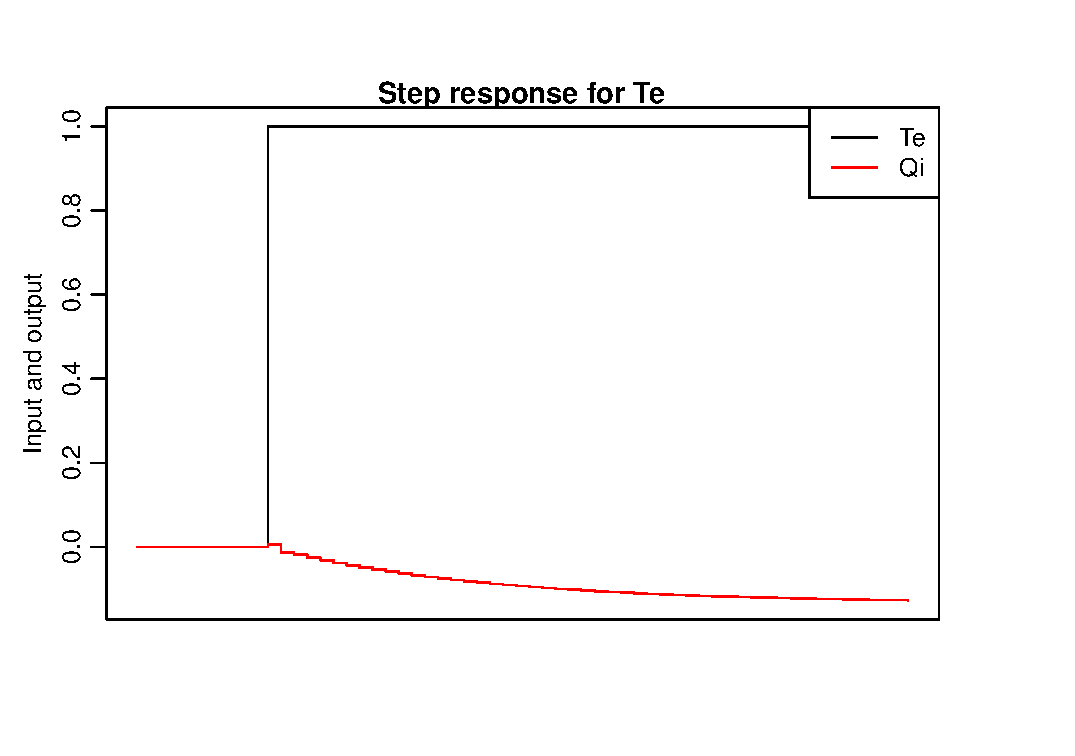
\includegraphics[width=0.8\textwidth]{../../../figures/StepResponse.eps}
    \caption{The step response for the temperature input for house 55. The red line converges towards a new constant level, which is the step response}
    \label{fig:StepResponse55}
\end{figure}


\noindent The different step responses without Fourier series for the houses are illustrated in \cref{fig:HCL}. For each house, the leftmost estimate is the one for the regression model on the daily data. The middle estimate is the one generated by the Marima found based on the BIC criterion. It can be seen that even though the estimate values are similar, the confidence interval is much wider for the Marima model. To get an estimate with a tighter confidence interval, another round of model selection is made, where the model with the smallest variance is chosen (the CL model), instead of basing the model selection on BIC. This is the rightmost estimate on the figure for each house. Compared to the BIC model, the CL model naturally provides more certain estimates, but they are still not as good as the ones for the regression model. For house 18 the difference is very big, but for house 55 and 6 the CL model is just slightly better.

\noindent \cref{fig:HCLF} shows the same estimates for the model with the Fourier series included. This improves some of the estimates. For house 55 and house 18 the overall performance is improved, but the estimates are still not as good as the regression model. House 55 seems to be the one where the certainty is closest to the regression model. But it still has a larger confidence interval, and the others are even worse. The step response estimates for the temperature with the CL model and with the Fourier series is listed in table... and the step response estimates for the solar radiation in ...  The solar radiation will not be compared to the regression model, because the parameters where not nearly as significant as the temperature, making the estimates unreliable. To summarize, the step response temperature estimates for the best model and the best house is still not as good as the regression model estimates for that house. The time series models simply cannot produce results that are as precise as the regression models.


\begin{figure}
    \centering
    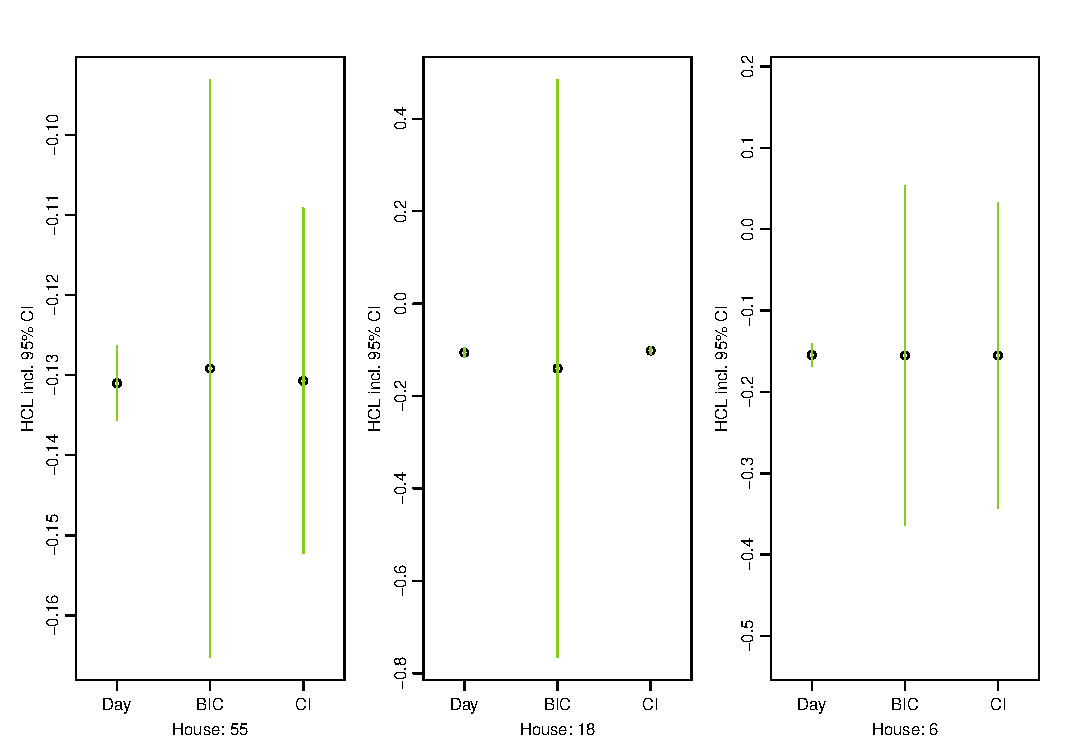
\includegraphics[width=0.8\textwidth]{../../../figures/MarimaHCL.eps}
    \caption{The temperature estimates from the regression models compared to the temperature step response for the Marima models without Fourier series. The regression model on the daily data is far superior. The Marima estimates are included for the models found based on BIC and the models with the smallest confidence interval.}
    \label{fig:HCL}
\end{figure}

\begin{figure}
    \centering
    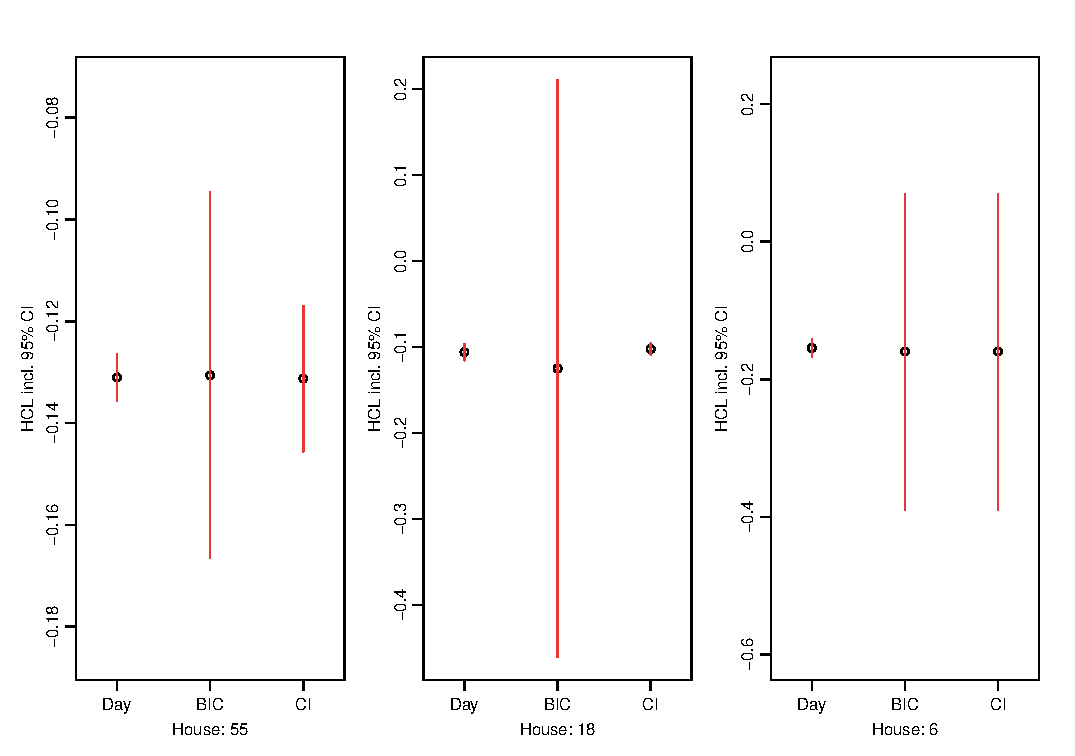
\includegraphics[width=0.8\textwidth]{../../../figures/MarimaHCLF.eps}
    \caption{The temperature estimates from the regression models compared to the temperature step response for the Marima models with Fourier series. There Fourier series does not improve the step response. The Marima estimates are included for the models found based on BIC and the models with the smallest confidence interval.}
    \label{fig:HCLF}
\end{figure}





\begin{table}[H]
    \centering
    \begin{tabular}{l|cccc}
    \hline
     & $\bm{\omega_{T}}$ & \textbf{Std. errors} & $\bm{2.5\%}$ & $\bm{97.5\%}$ \\ \hline \hline
    House 55 & 0.131 & 0.007 & 0.117 & 0.146 \\
    House 18 & 0.102 & 0.003 & 0.096 & 0.109 \\
    House 6  & 0.160 & 0.117 & -0.070 & 0.389\\
    \hline
    \end{tabular}
    \caption{}
    \label{tab: result_temp}
 \end{table}

 \begin{table}[H]
    \centering
    \begin{tabular}{l|cccc}
    \hline
     & $\bm{\omega_S}$ & \textbf{Std. errors} & $\bm{2.5\%}$ & $\bm{97.5\%}$ \\ \hline \hline
    House 55 & 0.0006 & 0.0003 & -6.21e-06 & 0.1318 \\
    House 18 & -0.0007 & 0.0001 & -0.0009 & 0.1026 \\
    House 6  & 0.0013 & 0.0069 & -0.0122 & 0.1732 \\
    \hline
    \end{tabular}
    \caption{}
    \label{tab: result_solar}
 \end{table}


